\documentclass{seg}
\usepackage{natbib}
\usepackage[left=1.0in, right=1.0in, top=1.0in, bottom=1.0in]{geometry}
\usepackage{algorithm}
\usepackage{algpseudocode}
\usepackage{booktabs}
\usepackage{multirow}
\usepackage{lineno}
\usepackage{setspace}
\doublespacing

\title{Python code for fast polyhedral full tensor gravity forward modelling}

\author{%
  Leyuan Wu$^{1}$ \and
  Chong Zhang$^{2}$\thanks{Corresponding author: zhangchong@cags.ac.cn} \and
  Longwei Chen$^{3}$\thanks{Corresponding author: longweichen\_glut@glut.edu.cn}
}

\begin{document}

\linenumbers

\maketitle

\begin{center}
    \footnotesize
    $^{1}$School of Physics and Optical Engineering, Zhejiang University of Technology, Hangzhou 310058, China \\
    $^{2}$China Deep Exploration Center (SinoProbe Center), Chinese Academy of Geological Sciences, Beijing 100037, China \\
    $^{3}$ Guangxi Key Laboratory of Exploration For Hidden Metallic Ore Deposits, College of Earth Sciences, Guilin University of Technology, Guilin 541006, China
\end{center}

\newpage

\begin{abstract}
Python code for fast polyhedral full tensor gravity forward modelling. Numba acceleration, suitable for local, regional, and global computations. Stable, accurate and efficient for very large meshes. Full gravity tensor, i.e., potential, first-order derivatives, and complete tensor of second-order derivatives. Two algorithmic variants: precomputed geometry for speed, on-the-fly geometry for memory efficiency. Validated against analytical solutions and Green's third identity on EROS shape model. Application to lunar topographic gravity potential with comparison to spherical harmonics. Open-source implementation for geophysical and planetary applications. 
\end{abstract}

\section{Introduction}

Polyhedral models have become a cornerstone in gravitational and magnetic field forward modelling due to their unique ability to represent sources with arbitrarily complex geometries-ranging from local topographic features to planetary-scale bodies such as asteroids and moons. Unlike simpler discretization schemes like rectangular prisms or tesseroids, which often introduce artificial discontinuities at interfaces, polyhedral models preserve the continuity and roughness of natural density or magnetization boundaries, thereby offering superior accuracy-particularly in the near-zone where high-frequency gravitational signals dominate 
\citep{Tsoulis2001JournalofGeodesy,Hikida2007Icarus,Benedek2018JGeod,Zhang2018JGeod,Hirt2019GeophysicalResearchLetters,Holzrichter2019Geophys.J.Int.,Saraswati2019JGeod}.

Over the past two decades, significant progress has been made in deriving space-domain analytical solutions for the gravitational potential, vector, and gradient tensor generated by polyhedral bodies. Early foundational work established closed-form expressions for homogeneous or linearly varying density distributions 
\citep{Barnett1976Geophysics,Okabe1979Geophysics,Holstein1996Geophysics,Werner1996CelestialMechDynAstr,Pohanka1998GeophysicalProspecting,Tsoulis2001Geophysics,Holstein2003Geophysics,Tsoulis2012Geophysics}, More recently, these formulations have been generalized to accommodate arbitrary polynomial density functions, enabling more realistic modelling of geophysical sources with heterogeneous internal structures \citep{DUrso2017SurvGeophys}. In particular, a series of works by \citet{Ren2017SurvGeophys,Ren2018GEOPHYSICS,Ren2020SurvGeophys,Ren2022GeophysicalResearchLetters} unified decades of prior results into a comprehensive analytical framework for both gravitational and magnetic fields of polyhedra with polynomial density or magnetization variations.

Beyond space-domain approaches, spectral methods have also played an important role. \citet{Jamet2020JGeod} introduced a novel and numerically stable method for computing spherical harmonic coefficients of the gravity field of a constant-density polyhedron by reducing volume integrals of solid harmonics to line integrals along the polyhedron’s edges. Spherical harmonic transform (SHT) based techniques, initiated by \citet{Wieczorek1998J.Geophys.Res.} as a spherical analog to the Cartesian method of \citet{Parker1973GeophysJInt}, enable efficient global topographic gravity modelling. However, solid spherical harmonic series suffer from divergence inside the Brillouin sphere-even for near-spherical large planets like Earth and Moon at high degrees-and are ill-suited for highly irregular bodies such as asteroids and comets \citep{Hu2015JGeod,Reimond2016JGRPlanets,Hirt2017JGRPlanets,Hirt2019GeophysicalResearchLetters,Bucha2019JGeod,Sprlak2021Earth-ScienceReviews}; spheroidal/ellipsoidal harmonics offer improved convergence at the expense of more complex parametrization and higher computational cost \citep{Wang2013JGeod,Claessens2013JGRSolidEarth,Rexer2016SurvGeophysa,Liu2025SurvGeophys}. 

Fourier-domain methods based on Cartesian Fast Fourier Transform (FFT) algorithms have also received significant attention in solving local modelling problems when a flat-earth approximation is applicable. Analytical wavenumber-domain formulations by \citet{Pedersen1978Geophysics}, \citet{1983WuXZ_CJG}, and \citet{Hansen1988Geophysics} laid the foundation for FFT-based polyhedral gravity forward modelling. Later, \citet{Wu2019JGeod,Wu2019JGeoda} developed efficient 2D/3D Fourier-domain algorithms that recast polyhedral gravity forward modelling-for bodies with constant or exponential density-into wavenumber-domain line integrals, leveraging Gauss-FFT and nonuniform FFT (NUFFT) techniques to achieve high computational accuracy, though computational cost still grows rapidly with model resolution due to the analytical evaluation of the spectrum. Recent adaptations of Parker`s method to general polyhedra further demonstrate the potential of spectral efficiency \cite{Wu2021J.Geophys.Res.SolidEarth}, yet space-domain formulations remain essential for validation and high-precision applications.

Accompanying these theoretical advances, several open-source implementations have become available. These include a FORTRAN implementation by \citet{Tsoulis2012Geophysics}, MATLAB routines introduced by \citet{Singh2001Geophysics} and later extended by \citet{Saraswati2019JGeod}, and a C\texttt{++} library (\url{https://github.com/zhong-yy/GraPly}) that implements the algorithms of \citet{Ren2017SurvGeophys,Ren2018GEOPHYSICS,Ren2020SurvGeophys,Ren2022GeophysicalResearchLetters}. However, practical experience with these codes reveals persistent numerical instabilities-particularly when evaluation points lie on or near polyhedral faces or vertices, and occasionally even at seemingly arbitrary locations (personal communication with \cite{Saraswati2019JGeod}). These issues highlight the continued need for a code that delivers consistent accuracy and reliability.

In this paper, we provide an open-source Python implementation for polyhedral gravity forward modelling based on the method introduced by \citet{Werner1996CelestialMechDynAstr}, which we find to be numerically stable, concise, and elegant. Two algorithmic variants are developed: one constructs an edge list from the face–vertex geometry and precomputes face and edge normals in memory to accelerate large-mesh computations; the other computes all geometric quantities on-the-fly, requiring significantly less memory and thus better suited for very large polyhedral meshes. Our implementation aims to serve both as a practical tool for geophysical and planetary applications and as a reliable reference for validating emerging spectral or data-driven methods.


\section{Methodology}

\subsection{Theoretical Framework}

We adopt the analytical formulation for the gravitational potential (GP), gravitational vector (GV), and gravity gradient tensor (GGT) of a homogeneous polyhedron as derived by \citet{Werner1996CelestialMechDynAstr}. This approach expresses all field components in terms of contributions from faces and edges, enabling efficient and numerically stable computation.

We assume the polyhedron is represented as a closed, manifold triangular mesh, composed of a set of vertices $\mathcal{V}$, a set of triangular faces $\mathcal{T}$, and a set of edges $\mathcal{E}$. Let $N_V = |\mathcal{V}|$, $N_T = |\mathcal{T}|$, and $N_E = |\mathcal{E}|$ denote their cardinalities. For a simply connected polyhedron, Euler's polyhedral formula gives $N_V + N_T - N_E = 2$, and since each triangle has three edges and each interior edge is shared by two faces, we have $N_E=1.5 N_T$ and $N_V \approx \tfrac{1}{2} N_T$, so all geometric complexities scale linearly with $N_T$.

For a polyhedron of constant density $\rho$, the gravitational potential $V$, gravitational vector $\mathbf{g} = \nabla V$, and gravity gradient tensor $\mathbf{T} = \nabla \nabla V$ at an observation point $P$ are given by \citep{Werner1996CelestialMechDynAstr}:

\begin{align}
V &= \frac{1}{2} G \rho \sum_{e \in \mathcal{E}} \mathbf{r}_e \cdot \mathbf{E}_e \cdot  
                         \mathbf{r}_e \; L_e 
    -\frac{1}{2} G \rho \sum_{t \in \mathcal{T}} \mathbf{r}_t \cdot \mathbf{F}_t \cdot   
                         \mathbf{r}_t \; \omega_t, \tag{1} \\
\mathbf{g} &= \nabla V = -G \rho \sum_{e \in \mathcal{E}} \mathbf{E}_e \cdot \mathbf{r}_e \; L_e 
           + G \rho \sum_{t \in \mathcal{T}} \mathbf{F}_t \cdot \mathbf{r}_t \; \omega_t, \tag{2} \\
\mathbf{T} &= \nabla \nabla V = G \rho \sum_{e \in \mathcal{E}} \mathbf{E}_e \; L_e 
                 - G \rho \sum_{t \in \mathcal{T}} \mathbf{F}_t \; \omega_t, \tag{3}
\end{align}
where $G = 6.67430 \times 10^{-11}~\mathrm{m^3\,kg^{-1}\,s^{-2}}$ is the gravitational constant. The vectors $\mathbf{r}_e$ and $\mathbf{r}_t$ denote position vectors from the observation point $P$ to representative points on edge $e$ and triangular face $t$, respectively. The geometric weighting factors $L_e$ and $\omega_t$ encode the influence of each edge and face, while $\mathbf{E}_e$ and $\mathbf{F}_t$ are dyadic tensors constructed from face and edge normals.

The face dyad $\mathbf{F}_t$ for a triangular face $t \in \mathcal{T}$ (oriented counter-clockwise with respect to the outward normal) is defined as:
\begin{equation}
\mathbf{F}_t = \hat{\mathbf{n}}_{t} \, \hat{\mathbf{n}}_{t}, \tag{4}
\end{equation}
where $\hat{\mathbf{n}}_{t}$ is the unit outward-pointing normal vector of face $t$.

Each interior edge $e \in \mathcal{E}$ is shared by two adjacent triangular faces $t^{+}$ and $t^{-}$, denote unit vectors along edge $e$ as $\hat{\mathbf{e}}^{+}$ and $\hat{\mathbf{e}}^{-}$ ($\hat{\mathbf{e}}^{+} = - \hat{\mathbf{e}}^{-}$), which are CCW in $t^{+}$ and $t^{-}$, respectively. The corresponding edge dyad $\mathbf{E}_e$ is:
\begin{equation}
\mathbf{E}_{e} = \hat{\mathbf{n}}_{t}^{+} \, \hat{\mathbf{n}}_{e}^{+} + \hat{\mathbf{n}}_{t}^{-} \, \hat{\mathbf{n}}_{e}^{-}, \tag{5}
\end{equation}
where $\hat{\mathbf{n}}_{e}^{+}$ and $\hat{\mathbf{n}}_{e}^{-}$ are unit edge-normal vectors lying in the planes of their respective faces and perpendicular to the edge direction:
\[
\hat{\mathbf{n}}_{e}^{+} = \hat{\mathbf{e}}^{+} \times \hat{\mathbf{n}}_{t}^{+}, \quad
\hat{\mathbf{n}}_{e}^{-} = \hat{\mathbf{e}}^{-} \times \hat{\mathbf{n}}_{t}^{-}.
\]

The scalar geometric factors depend only on the relative geometry between the observation point $P$ and the polyhedral element. For an edge $AB$, the per-edge factor $L_e$ is:
\begin{equation}
L_e = \ln \left( \frac{r_{PA} + r_{PB} + e_{AB}}{r_{PA} + r_{PB} - e_{AB}} \right), \tag{6}
\end{equation}
where $r_{PA} = \|\mathbf{r}_{PA}\|$, $r_{PB} = \|\mathbf{r}_{PB}\|$, and $e_{AB} = \|\mathbf{r}_{AB}\|$ are the Euclidean distances from $P$ to vertices $A$ and $B$, and the length of edge $AB$, respectively.

For a triangular face $ABC$, the per-face solid angle factor $\omega_t$ is:
\begin{equation}
\omega_t = 2 \arctan \left( 
\frac{
\mathbf{r}_{PA} \cdot (\mathbf{r}_{PB} \times \mathbf{r}_{PC})
}{
r_{PA} r_{PB} r_{PC} 
+ r_{PA} (\mathbf{r}_{PB} \cdot \mathbf{r}_{PC}) 
+ r_{PB} (\mathbf{r}_{PC} \cdot \mathbf{r}_{PA}) 
+ r_{PC} (\mathbf{r}_{PA} \cdot \mathbf{r}_{PB})
} \right), \tag{7}
\end{equation}
which represents the signed solid angle subtended by the face at point $P$.

This formulation provides a unified, closed-form description of the full gravity tensor (potential, vector, and gradient) and serves as the foundation for our efficient and robust Python implementation.

\subsection{Algorithm Design and Benchmark}

We provide two Numba-accelerated implementations of the Werner--Schmidt polyhedral gravity formulation \citep{Werner1996CelestialMechDynAstr}, tailored for triangular meshes $(\mathcal{V}, \mathcal{T})$. Both compute the gravitational potential $V$, vector $\mathbf{g}$, and gradient tensor $\mathbf{T}$ from vertex coordinates and face indices, with inputs in km, density $\rho$ in $\mathrm{kg/m^3}$, and outputs scaled to geophysical units ($V$ in $\mathrm{m^2/s^2}$, $\mathbf{g}$ in mGal, and $\mathbf{T}$ in Eotvos).

\subsubsection*{Version 1: Precomputed Geometry}
This variant precomputes all static geometric data once per mesh:
\begin{itemize}
    \item Constructs a global edge list $\mathcal{E}$ storing adjacent faces and orientation.
    \item Computes unit face normals $\hat{\mathbf{n}}_t$ for all $t \in \mathcal{T}$ and corresponding edge normals $\hat{\mathbf{n}}_{e}^{\pm}$ in parallel.
\end{itemize}
During evaluation, each observation point accumulates contributions from solid angles $\omega_t$ (faces) and logarithmic edge factors $L_e$ (edges). This minimizes arithmetic overhead and is optimal for repeated evaluations or moderate meshes ($N_T \lesssim 10^8$), at the cost of approximately $164\,N_T$ bytes of memory (e.g., $\sim\!16$~GB for $N_T = 10^8$).

\begin{algorithm}[H]
\small
\caption{WerSch\_numba\_v1 (Precomputed Geometry)}
\begin{algorithmic}[1]
\Require Observation points $\mathbf{P}$, vertices $\mathcal{V}$, faces $\mathcal{T}$, density $\rho$
\Ensure $V(\mathbf{P})$, $\mathbf{g}(\mathbf{P})$, $\mathbf{T}(\mathbf{P})$ in geophysical units

\State $\mathcal{E} \gets \Call{BuildEdgeList}{\mathcal{T}}$
\State $(\hat{\mathbf{n}}_t)_{t \in \mathcal{T}} \gets \Call{ComputeFaceNormals}{\mathcal{V}, \mathcal{T}}$
\State $(\hat{\mathbf{n}}_{e}^{+}, \hat{\mathbf{n}}_{e}^{-})_{e \in \mathcal{E}} \gets \Call{ComputeEdgeNormals}{\mathcal{V}, \mathcal{E}, \hat{\mathbf{n}}_t}$

\ForAll{$\mathbf{p} \in \mathbf{P}$} \textbf{in parallel}
    \State Initialize accumulators for $V$, $\mathbf{g}$, $\mathbf{T}$
    
    \ForAll{$t \in \mathcal{T}$}
        \State Compute solid angle $\omega_t(\mathbf{p})$
        \State Accumulate face contribution to $V$, $\mathbf{g}$, $\mathbf{T}$
    \EndFor
    
    \ForAll{$e \in \mathcal{E}$}
        \State Compute logarithmic factor $L_e(\mathbf{p})$
        \State Accumulate edge contribution to $V$, $\mathbf{g}$, $\mathbf{T}$
    \EndFor
    
    \State Apply unit scaling to geophysical conventions
\EndFor
\end{algorithmic}
\end{algorithm}

\subsubsection*{Version 2: On-the-Fly Geometry}
To reduce memory footprint, all geometric quantities are computed during evaluation:
\begin{itemize}
    \item Face normals $\hat{\mathbf{n}}_t$ are computed per triangle.
    \item Edge normals are derived on the fly via $\hat{\mathbf{n}}_{e} = \hat{\mathbf{e}} \times \hat{\mathbf{n}}_t$.
\end{itemize}
No global edge list is stored; each interior edge is processed twice (once per adjacent face), with contributions accumulating correctly due to the linearity of the formulation. Memory usage is only $\sim\!24\,N_T$ bytes (e.g., $\sim\!2.4$~GB for $N_T = 10^8$), and can be further reduced by partitioning $\mathcal{T}$ into chunks-ideal for extreme-scale models ($N_T \gg 10^8$).

\begin{algorithm}[H]
\small
\caption{WerSch\_numba\_v2 (On-the-Fly Geometry)}
\begin{algorithmic}[1]
\Require $\mathbf{P}$, $\mathcal{V}$, $\mathcal{T}$, $\rho$
\Ensure $V(\mathbf{P})$, $\mathbf{g}(\mathbf{P})$, $\mathbf{T}(\mathbf{P})$ in geophysical units

\ForAll{$\mathbf{p} \in \mathbf{P}$} \textbf{in parallel}
    \State Initialize accumulators for $V$, $\mathbf{g}$, $\mathbf{T}$
    
    \ForAll{$t \in \mathcal{T}$}
        \State Compute $\hat{\mathbf{n}}_t$
        \State Compute $\omega_t(\mathbf{p})$, accumulate face terms
        
        \ForAll{edge $e$ of triangle $t$}
            \State Compute $\hat{\mathbf{e}}$
            \State Compute $\hat{\mathbf{n}}_e \gets \hat{\mathbf{e}} \times \hat{\mathbf{n}}_t$
            \State Compute $L_e(\mathbf{p})$, accumulate edge terms
        \EndFor
    \EndFor
    
    \State Apply unit scaling to geophysical conventions
\EndFor
\end{algorithmic}
\end{algorithm}

Both versions employ numerically stable evaluation (\texttt{atan2}-based solid angle computation, safeguarded logarithms for $L_e$) and leverage Numba’s parallel JIT compilation. Version~1 is recommended for speed-critical scenarios with repeated evaluations, and Version~2 is more suitable for memory-constrained or large-scale modelling where $N_T \gg 10^8$.

We benchmark \texttt{WerSch\_numba\_v1} and \texttt{WerSch\_numba\_v2} to validate their numerical equivalence and compare performance. The test uses a homogeneous sphere ($R = 1.0$~km, $\rho = 2670~\mathrm{kg/m^3}$) discretized by recursive icosahedral subdivision, with field evaluations at quasi-uniform points on a concentric sphere ($r_{\mathrm{obs}} = 1.1$~km). This creates a matrix of problems from $N_T, N_P = 20$ up to $\approx 1.3 \times 10^6$.

As shown in Figure~\ref{fig:Benchmark}, the results confirm that both algorithms are numerically identical for practical purposes. The maximum absolute differences are negligible: for the vertical gravity component ($g_z$), they range from $10^{-14}$ to $10^{-11}$~mGal against a reference standard deviation of $35.62$~mGal; for the vertical gradient $T_{zz}$, differences are between $10^{-13}$ and $10^{-10}$~Eotvos against a standard deviation of $501.61$~Eotvos.

In terms of performance, \texttt{v1} is consistently faster for moderate-to-large problems, with the runtime ratio $t_2/t_1$ stabilizing near 1.3--1.5 for the largest configurations. However, \texttt{v2} has a significantly smaller memory footprint due to its on-the-fly computation. This makes \texttt{v2} a robust alternative not only for small-scale tests but also for extremely large problems where memory constraints would otherwise prevent the use of precomputed edge-based data structures. Thus, the choice between versions hinges on the trade-off between computational speed (\texttt{v1}) and memory efficiency (\texttt{v2}).

\section{Numerical examples}

\subsection{An ideal sphere test}

We validate our polyhedral forward modelling implementation using a homogeneous sphere-a canonical test case with a known analytical solution for the gravitational potential, vector, and gradient tensor. We compare two standard approaches for discretizing a spherical surface into triangular polyhedra: recursive icosahedral subdivision \citep{Zhang2018JGeod} and triangulation of a regular longitude--latitude (geographic) grid. Both are widely used in geophysical modelling, though they differ in geometric structure, convergence behaviour, and compatibility with existing datasets.

The icosahedral method generates meshes with nearly equilateral triangles and minimal variation in edge lengths across the sphere. As shown in Figure~\ref{fig:Sphere_Polyhedron} (top row) and quantified in Table~\ref{tab:ico_geo_sphere}, this leads to rapid and balanced convergence in both surface area and volume errors as the refinement level $n$ increases. For instance, at $n=6$ ($N_T = 81920$), the relative area error is already below $10^{-4}$, and the ratio of maximum to minimum edge length remains close to $1.5$.

In contrast, the geographic grid-while intuitive and aligned with many raster-based geospatial datasets (e.g., digital elevation models, or gravity models on regular grids)-exhibits strong meridian convergence at the poles. This results in highly elongated triangles near the poles and a wide spread in edge lengths, clearly visible in the bottom row of Figure~\ref{fig:Sphere_Polyhedron}. At the same refinement level ($n=6$), the shortest edges are about two orders of magnitude smaller than the longest ones (see Table~\ref{tab:ico_geo_sphere}), which may pose challenges for numerical stability in forward modelling if not properly addressed.

Nevertheless, both discretizations converge systematically toward the ideal sphere. As $n$ increases beyond 8, geometric errors in both area and volume fall below $10^{-5}$ for both methods (Table~\ref{tab:ico_geo_sphere}), confirming that either approach can achieve high geometric fidelity given sufficient resolution. The choice between them thus involves practical trade-offs: icosahedral meshes offer superior geometric regularity and are well-suited for global, high-precision modelling, whereas geographic grids provide straightforward compatibility with structured observational data and simpler indexing for regional applications.

To assess the impact of these geometric differences on gravity forward modelling, we compute the full gravity tensor-comprising the potential $V$, the gravitational acceleration vector in the North-East-Downward (NED) (local north-oriented coordinate system), and all independent components of the gravity gradient tensor-using our \texttt{WerSch\_numba\_v2} implementation on both mesh types. These results are compared against the analytical solution for a homogeneous sphere of radius $R = 6371.393~\mathrm{km}$ and density $\rho = 5520~\mathrm{kg/m^3}$. Observations are placed at four altitudes above the surface ($h = 0.001$, $0.1$, $1$, and $10~\mathrm{km}$), with 5000 quasi-uniform points per altitude generated via Fibonacci sampling.

Figure~\ref{fig:IcoGeoSphere_Global} shows the relative $L_2$ errors for selected field components as a function of mesh resolution. Both discretizations converge toward the analytical solution as $N_T$ increases, with errors decreasing monotonically across all altitudes. At comparable resolutions, the icosahedral discretization consistently yields marginally lower errors, reflecting its more uniform geometry. As expected, errors are largest in the near-field ($h = 0.001~\mathrm{km}$) and diminish rapidly with altitude due to the smoothing effect of the Newtonian potential. Importantly, the gravity field discrepancies align with the underlying geometric approximation errors reported in Table~\ref{tab:ico_geo_sphere}: since both the analytical sphere and the polyhedral formulation are exact for their respective domains, the observed differences arise primarily from how closely the polyhedral surface approximates the ideal sphere. This confirms that our implementation operates at machine precision, and that the dominant source of error is geometric-not algorithmic.

\subsection{EROS shape model test}

We validate our polyhedral implementation by numerically testing Green's third identity \citep{Blakely1995} on the asteroid 433 EROS shape model \citep{Gaskell2020a}. The gravitational potential at any exterior point $\mathbf{r}$ can be reconstructed from the potential and its normal derivative on the body’s surface $S$:

\begin{equation}
\begin{split}
V(\mathbf{r}) &= \frac{1}{4\pi} \oint_S 
\left[ V(\tilde{\mathbf{r}}) \frac{\partial}{\partial \tilde{n}} 
\left( \frac{1}{|\mathbf{r} - \tilde{\mathbf{r}}|} \right)
    - \frac{1}{|\mathbf{r} - \tilde{\mathbf{r}}|} 
    \frac{\partial V(\tilde{\mathbf{r}})}{\partial \tilde{n}} \right] dS \\
&\approx \sum_{i=1}^{N_T} s_i 
\Big[ V(\tilde{\mathbf{r}}_{i}) \mathcal{G}_{\tilde{n}} (\mathbf{r},\tilde{\mathbf{r}}_{i})
    - \mathcal{G}(\mathbf{r},\tilde{\mathbf{r}}_{i}) g_{\tilde{n}}(\tilde{\mathbf{r}}_{i}) \Big],
\end{split}
\tag{8}
\label{eq:green3}
\end{equation}
where $\mathcal{G}(\mathbf{r},\tilde{\mathbf{r}}) = \frac{1}{4\pi |\mathbf{r} - \tilde{\mathbf{r}}|}$ is the Green’s function, $\mathcal{G}_{\tilde{n}} (\mathbf{r},\tilde{\mathbf{r}}_{i})$ denotes its first-order outer normal derivative evaluated at the center $\tilde{\mathbf{r}}_i$ of triangular facet $S_i$, $s_i$ is the area of $S_i$, and $g_{\tilde{n}}(\tilde{\mathbf{r}}_{i}) = \partial V / \partial \tilde{n}$ is the outward normal component of the gravity vector at $\tilde{\mathbf{r}}_i$. This representation provides a powerful consistency check: if both $V$ and $g_{\tilde{n}}$ are computed accurately on the surface, the reconstructed potential $V(\mathbf{r})$ should converge to the true value as the mesh is refined.

Using the EROS shape model (856 vertices, 1708 faces) and a constant density of $\rho = 2670~\mathrm{kg/m^3}$, we compute $V$ and $g_{\tilde{n}}$ at all facet centers via \texttt{WerSch\_numba\_v1}. We then evaluate Equation~\eqref{eq:green3} on three concentric spheres of radii $r = 17.8$, $18.0$, and $20.0$~km, comparing the result against a reference solution obtained by direct polyhedral forward modelling. The EROS mesh is progressively refined using linear subdivision; at subdivision level $n$, the number of triangular faces grows as $N_T = 1708 \times 4^n$, reaching $N_T \approx 7 \times 10^6$ at $n = 6$. This refinement process, illustrated in Fig.~\ref{fig:EROS_Geometry}, preserves geometric fidelity while increasing surface resolution.

As expected, the approximation error decreases systematically with refinement, confirming both the correctness of our field computations and the validity of Green`s third identity applied to potential fields caused by complex polyhedral bodies. Figure~\ref{fig:EROS_ErrorMaps} shows the spatial distribution of relative errors on the innermost evaluation sphere ($r = 17.8$~km) for four refinement levels. At coarse resolutions, errors are elevated near the positive and negative $x$-axis—regions where EROS is most elongated and closest to the evaluation surface. Importantly, this spatial pattern persists even at the highest refinement level: although the magnitude of the relative error drops below $10^{-5}$, the residual errors remain concentrated near the tips along $\pm x$. This indicates that the error structure is not an artifact of poor discretization but reflects the intrinsic sensitivity of the near-field potential to local geometry. The global convergence trend is quantified in Fig.~\ref{fig:EROS_Convergence}, where both RMS and maximum relative errors decrease by over three orders of magnitude as the mesh is refined.

\subsection{Lunar topographic gravitational potential test}

To further validate our polyhedral implementation at planetary scale, we compute the topographic gravitational potential (TGP) of the Moon using both spherical harmonics (SH) and polyhedral (PH) methods. The lunar shape is modelled using the LOLA spherical harmonic model \texttt{Moon\_shape\_719.sh} downloaded from \citet{Wieczorek2024}, truncated to degree~$359$, which corresponds to a Driscoll–Healy (DH2) equi-sampled latitude/longitude grid of resolution~$15^{\prime}$ (arc-minute) \citep{Driscoll1994AdvancesinAppliedMathematics,Wieczorek2018GeochemGeophysGeosyst}. The topographic model is then obtained by subtracting from the shape model a reference radius of $r_{\mathrm{ref}} = 1737.151$~km—the mean value of the degree-$359$ SH shape model. A constant crustal density of $\rho = 2560~\mathrm{kg/m^3}$ is assumed.

In the SH approach, implemented via \texttt{pyshtools} \citep{Wieczorek2018GeochemGeophysGeosyst}, the topographic potential is computed up to $n_{\max}=7$ in the binomial expansion of the topography \citep{Wieczorek1998J.Geophys.Res.}, yielding a gravity field expanded to degree~$l_{\max} = 2519$. The resulting gravity vector components ($g_x, g_y, g_z$) are evaluated on a $15^{\prime} \times 15^{\prime}$ grid on the sphere of radius $r_{\mathrm{calc}} = 1748.0$~km, which lies safely above the maximum topography of the applied lunar shape model. Extending $n_{\max}$ to higher orders would further improve the accuracy of the SH method, but is limited by numerical instabilities in \texttt{pyshtools} for spherical harmonic expansions beyond degree~$2800$. We examine results obtained using $n_{\max}$ from~$1$ to~$7$; the incremental contribution beyond $n_{\max}=7$ is negligible, with maximum discrepancies below~$1$~mGal and standard deviations under~$0.1$~mGal. Thus, $n_{\max}=7$ provides a stable and sufficiently accurate SH reference for comparison with our polyhedral solutions.

For the PH method, the same shape model is converted into triangular meshes based on geographic grids with resolutions of~$15^{\prime}$ ($N_{T}=2\,070\,720$) and~$6^{\prime}$ ($N_{T}=12\,952\,800$). The forward modelling is performed using our \texttt{WerSch\_numba\_v1} algorithm, with observation points placed on the same $15^{\prime} \times 15^{\prime}$ grid at $r_{\mathrm{calc}} = 1748.0$~km. The topographic gravity signal is isolated by subtracting the gravity field of a homogeneous sphere of radius~$r_{\mathrm{ref}}$ and density~$\rho$ from the polyhedral solution of the full shape model.

Table~\ref{tab:Moon_SH_PH_comparison} summarizes the statistical comparison between the two methods. At $15$-arcmin resolution, the PH solution agrees with the SH reference to within $0.7$~mGal (north, $g_x$), $0.8$~mGal (east, $g_y$), and $1.1$~mGal (downward, $g_z$) in standard deviation, with maximum differences of $-13.2$, $-14.8$, and $-21.5$~mGal, respectively. At $6$-arcmin resolution, agreement improves markedly across all components: standard deviations drop to $0.1-0.2$~mGal and maximum errors fall below $3.4$~mGal, confirming that residual discrepancies stem from geometric discretization rather than algorithmic inaccuracies.

Figure~\ref{fig:Moon_TopoGz_PH_vs_SH_2} visualizes the global distribution of these differences. The top-left panel shows lunar topography, with white triangles indicating locations of the largest $g_z$ discrepancies in the $15$-arcmin PH-SH comparison; these sites were selected to be at least $1000$~km apart to ensure spatial independence. The top-right panel displays the SH-derived $g_z$ field, while the bottom-left and bottom-right panels show the difference $g_z^{\mathrm{ph}} - g_z^{\mathrm{sh}}$ for the $15$- and $6$-arcmin PH models, respectively. Since the input shape model is a continuous spherical harmonic representation, the polyhedral method requires a discrete mesh approximation—introducing resolution-dependent errors that diminish as the mesh is refined. The resulting error pattern is spatially coherent and decreases significantly with finer resolution.

To quantify convergence, we evaluate the gravity field at the ten sites labelled A-J in Figure~\ref{fig:Moon_TopoGz_PH_vs_SH_2}, which exhibit the largest $|g_z|$ discrepancies in the $15$-arcmin PH-SH comparison. Figure~\ref{fig:Moon_TopoGxyz_PH_vs_SH_3} shows the absolute errors in all three gravity components ($g_x$, $g_y$, $g_z$) as a function of polyhedral mesh resolution, ranging from $15$ to $1$ arcminute. Since the input lunar shape is a continuous spherical harmonic model, its discretization into a polyhedral mesh introduces resolution-dependent geometric errors; as the mesh is refined, these errors generally diminish. The gravity errors decrease monotonically with increasing resolution and fall below $1$~mGal (dashed line) for resolutions finer than $\sim\!5$ arcminutes in most cases. However, at the finest resolution (1 arcminute), the error reduction plateaus or slightly increases for a few locations—most notably point A—suggesting that the SH reference solution, truncated at degree $n_{\text{max}} = 7$, may be approaching its intrinsic accuracy limit, which is on the order of $1$~mGal at certain sites. These computations employ algorithm \texttt{WerSch\_numba\_v2}, which is optimized for large-mesh, few-observation scenarios. Overall, this behaviour confirms the numerical consistency of our polyhedral implementation and its convergence toward the SH solution as the surface approximation improves.

\section{Conclusion}

\section{Acknowledgments}
This study was funded by the National Natural Science Foundation of China (Grant No. 42474184, 42374172, 42374173). This work utilized several open-source Python packages, including PyVista \citep{Sullivan2019JOSS}, PyGMT \citep{Wessel2019GeochemGeophysGeosyst}, and pyshtools \citep{Wieczorek2018GeochemGeophysGeosyst}, for data processing and visualization.

\section{Data and Materials Availability}
All related Python code and Jupyter notebooks to reproduce all the numerical results in this work can be found at figshare: \url{https://figshare.com/}.


\clearpage
\begin{figure}
    \centering
    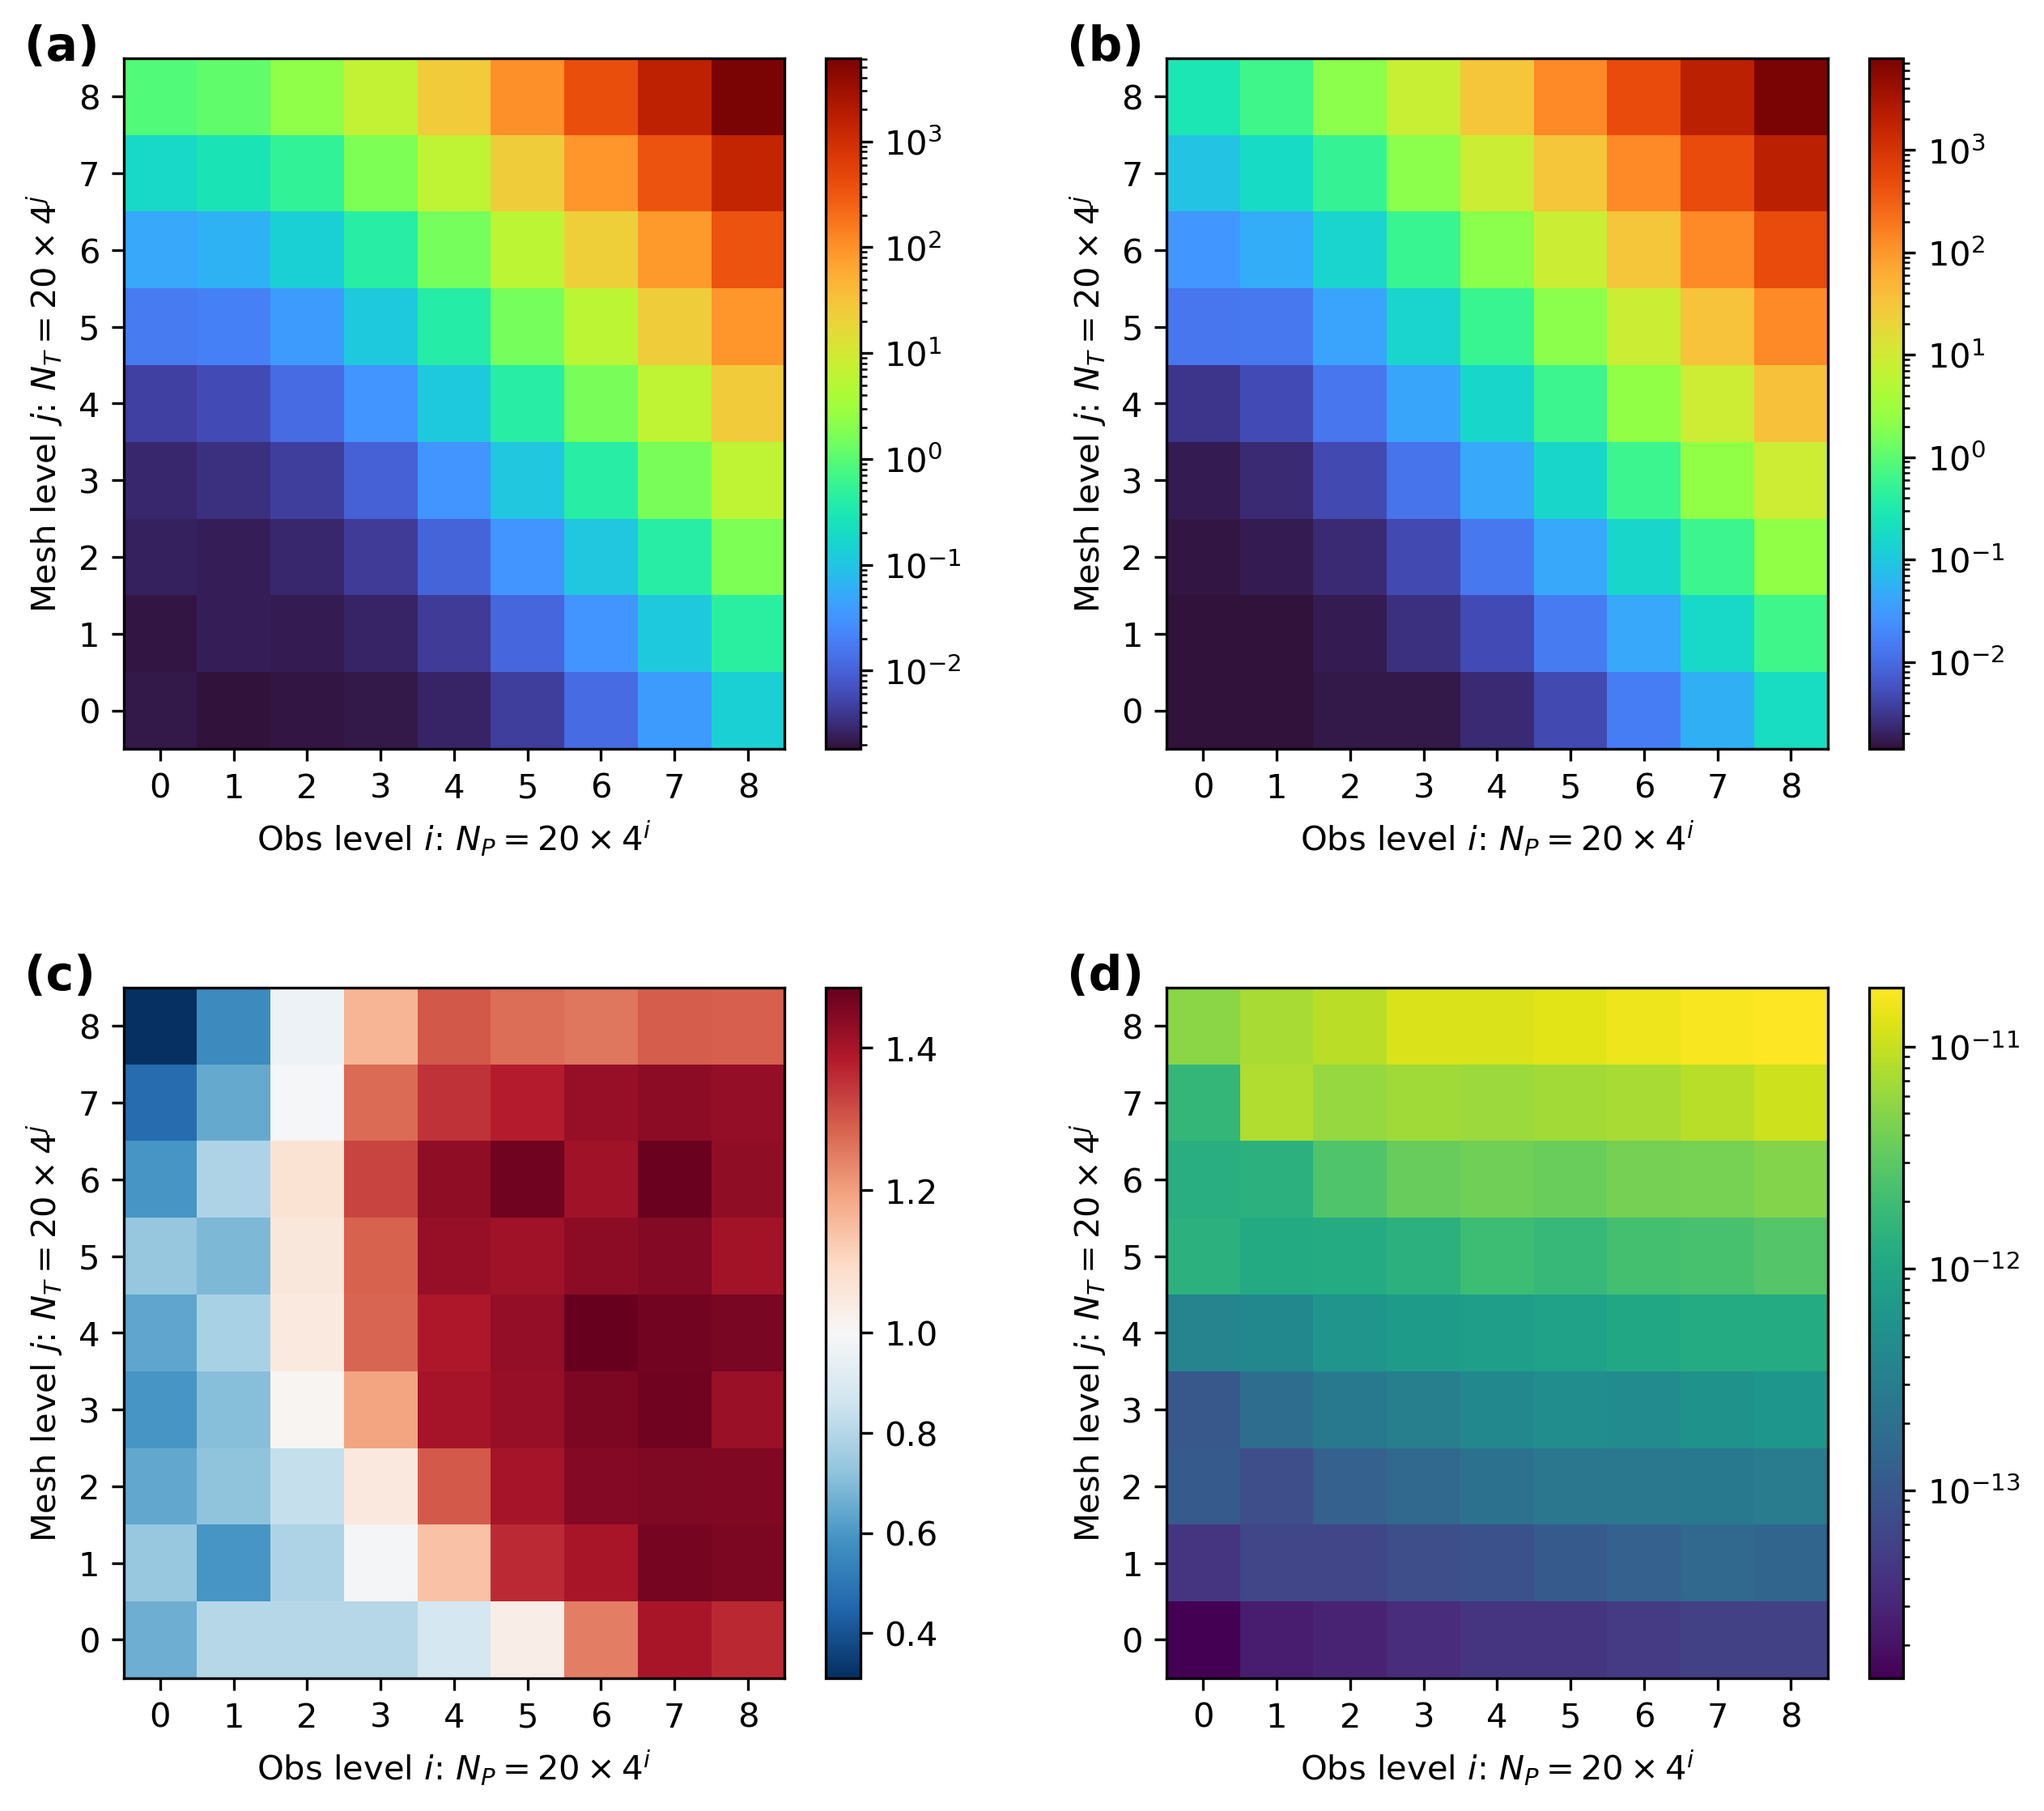
\includegraphics[width=0.95\textwidth]{Figs/Benchmark_WerSch_v1v2_nsub8.png}
    \caption{Benchmark of \texttt{WerSch\_numba\_v1} and \texttt{WerSch\_numba\_v2}. The source body is a unit sphere ($R = 1.0$ km) with constant density $\rho = 2670~\mathrm{kg/m^3}$, discretized by recursive icosahedral subdivision, yielding $N_T = 20 \times 4^{j}$ triangular faces for refinement level $j = 0, \dots, 8$. Observation points are placed on a concentric sphere of radius $r_{\mathrm{obs}} = 1.1$ km using Fibonacci sphere sampling, with $N_P = 20 \times 4^{i}$ points for level $i = 0, \dots, 8$. Shown from top-left to bottom-right: (a) runtime of Version~1 (sec), (b) runtime of Version~2, (c) runtime ratio $t_2/t_1$, and (d) maximum absolute difference in the computed vertical gravity component $g_z$ (mGal) between the two versions.}
    \label{fig:Benchmark}
\end{figure}

\clearpage
\begin{figure}
    \centering
    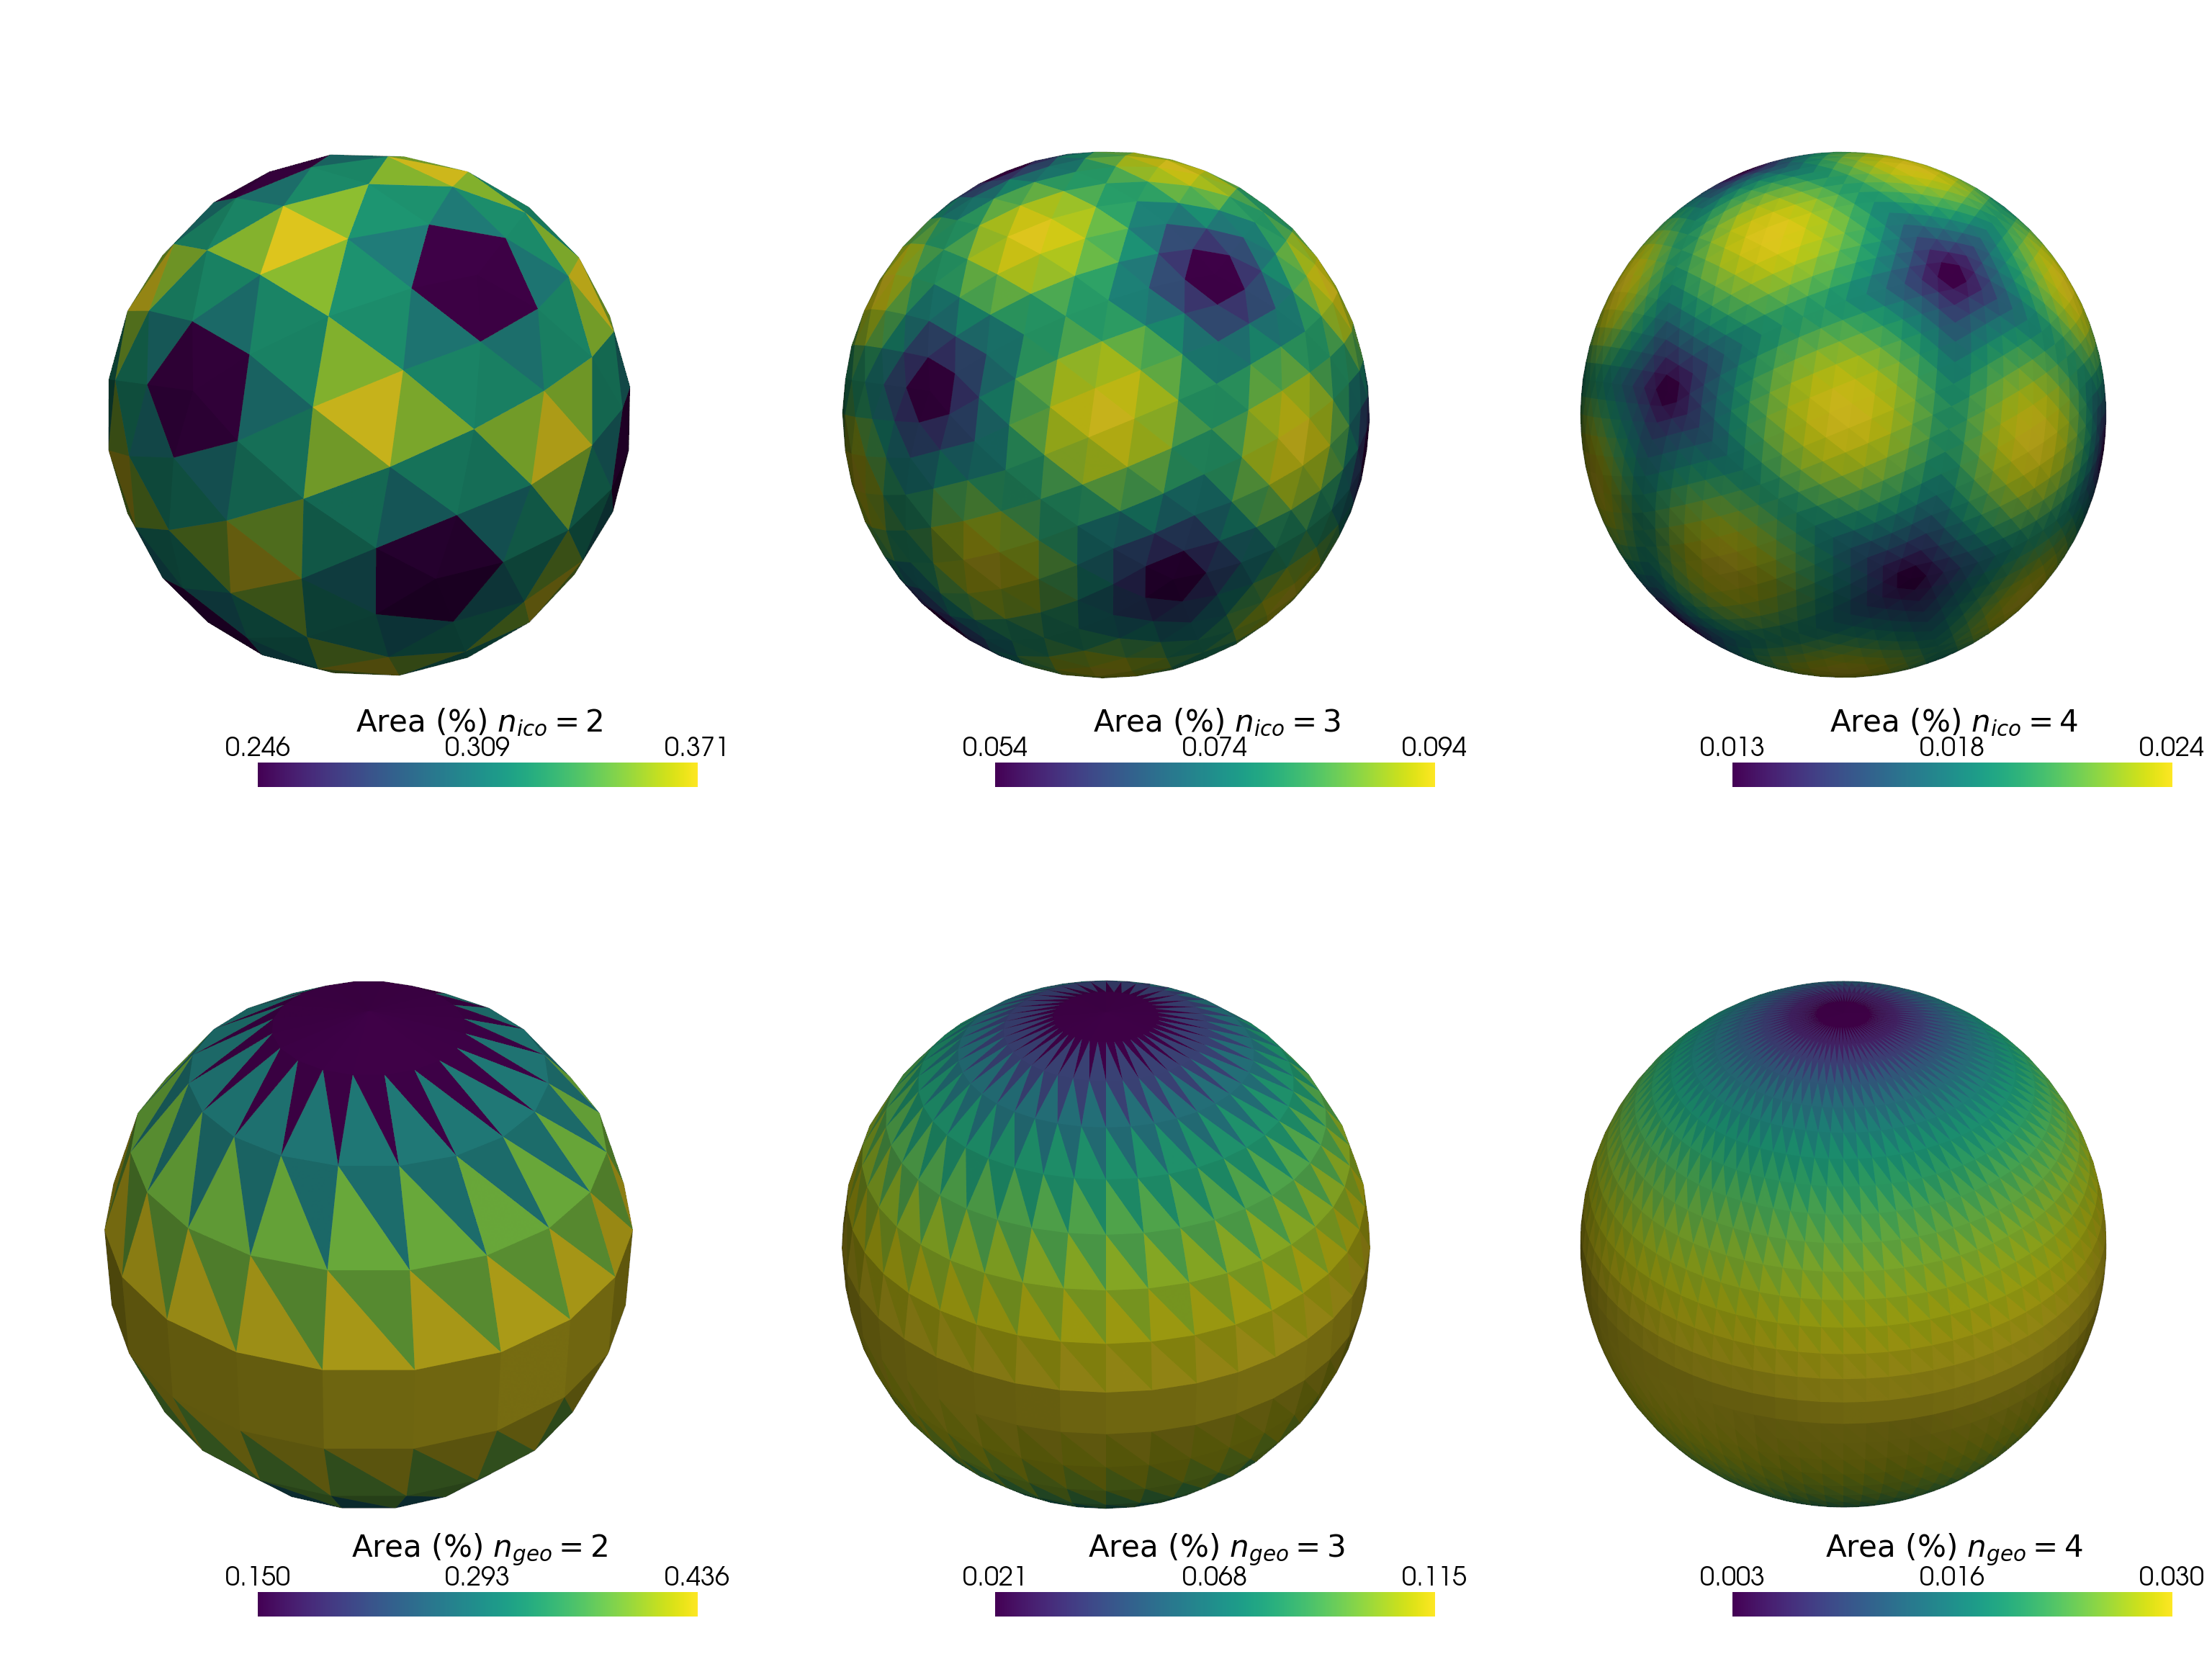
\includegraphics[width=0.95\textwidth]{Figs/Sphere_Polyhedron.png}
    \caption{Two common strategies for polyhedral approximation of a unit sphere: (top row) recursive subdivision of an icosahedron and (bottom row) triangulated regular geographic grid. Meshes at refinement levels $n = 2, 3, 4$ are shown, colored by the relative area of each triangular face (\% of total surface area). The icosahedral meshes exhibit more uniform element sizes, while the geographic grids show pronounced polar clustering, leading to high variability in triangle areas-particularly near the poles.}
    \label{fig:Sphere_Polyhedron}
\end{figure}

\clearpage
\begin{figure}
    \centering
    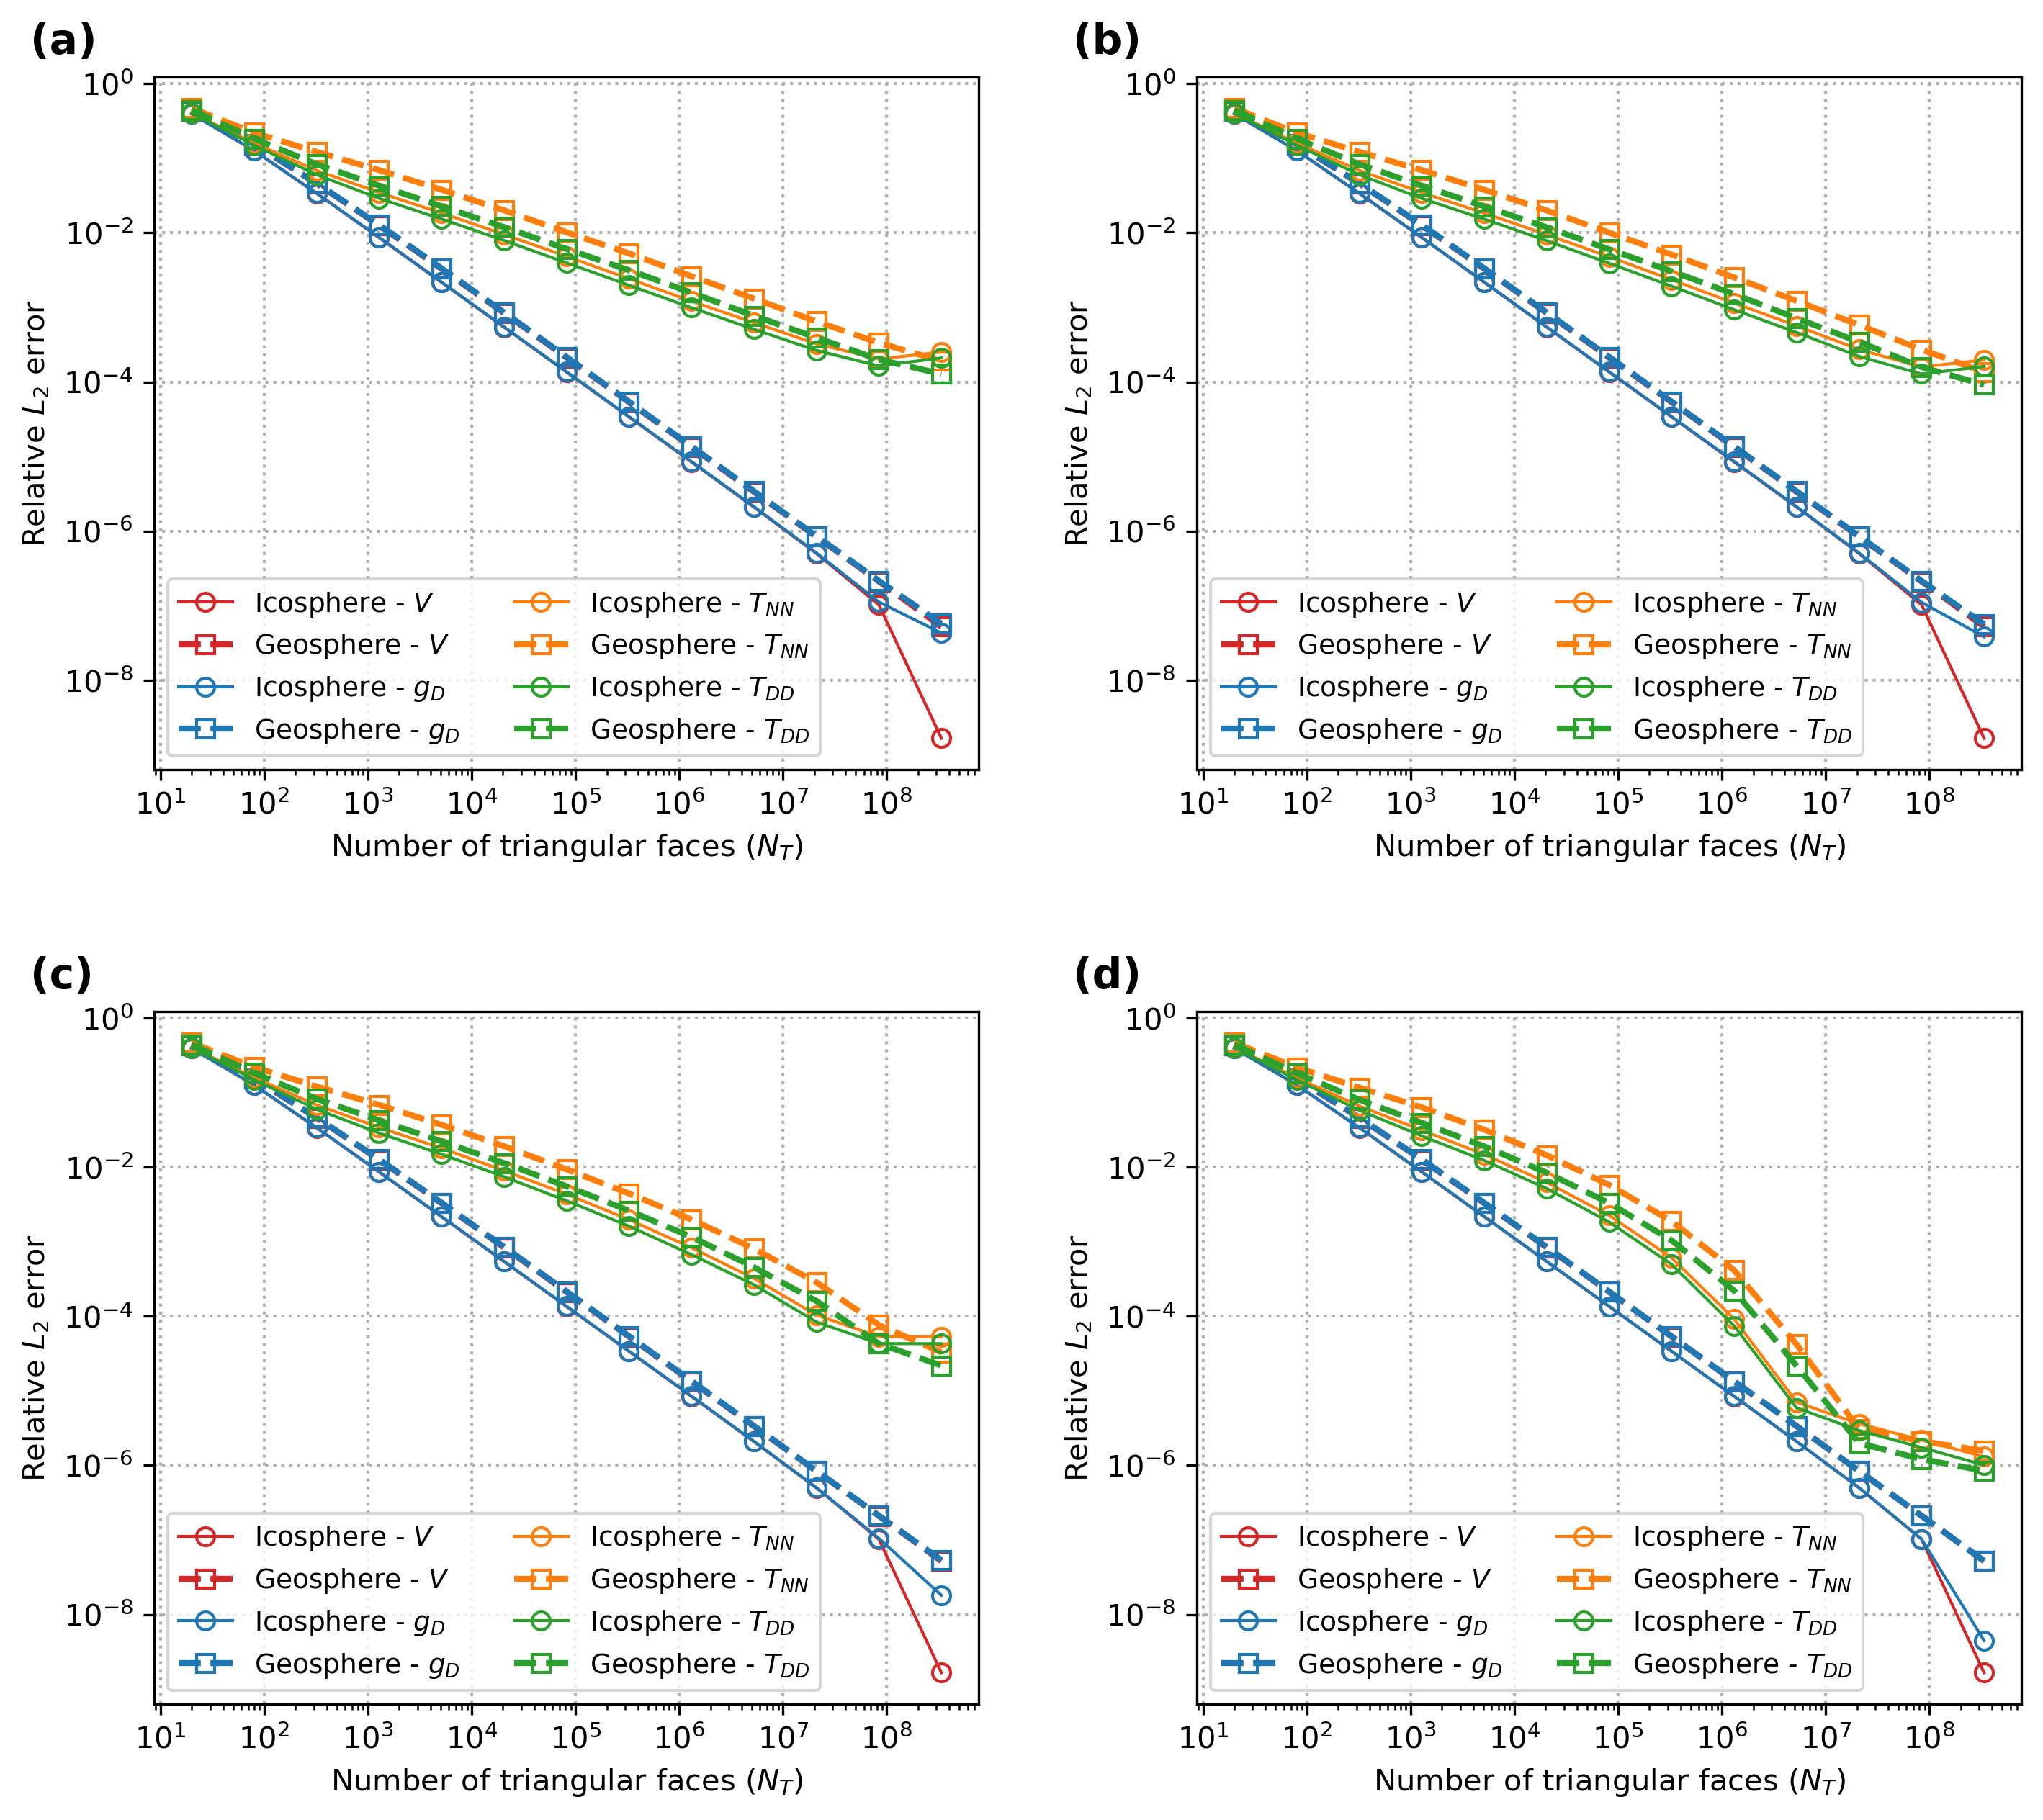
\includegraphics[width=0.95\textwidth]{Figs/IcoGeoSphere_Global_nsub12_nobs5000.png}
    \caption{Convergence of polyhedral gravity solutions toward the analytical field of a homogeneous Earth-sized sphere. Relative $L_2$ errors in selected field components (potential $V$, down-component $g_D$, and diagonal gradients $T_{NN}$, $T_{DD}$) are shown as functions of mesh resolution ($N_T =$ number of triangular faces). Panels correspond to different observation altitudes: (a)~0.001~km, (b)~0.1~km, (c)~1~km, and (d)~10~km. Solid lines with open circles represent icosahedral discretizations; dashed lines with open squares denote geographic (longitude--latitude) grids. Both methods converge with increasing resolution, with errors decreasing more rapidly at higher altitudes. The agreement between the two formulations confirms that discrepancies are due to geometric approximation rather than numerical computation.}
    \label{fig:IcoGeoSphere_Global}
\end{figure}

\clearpage
\begin{figure}
    \centering
    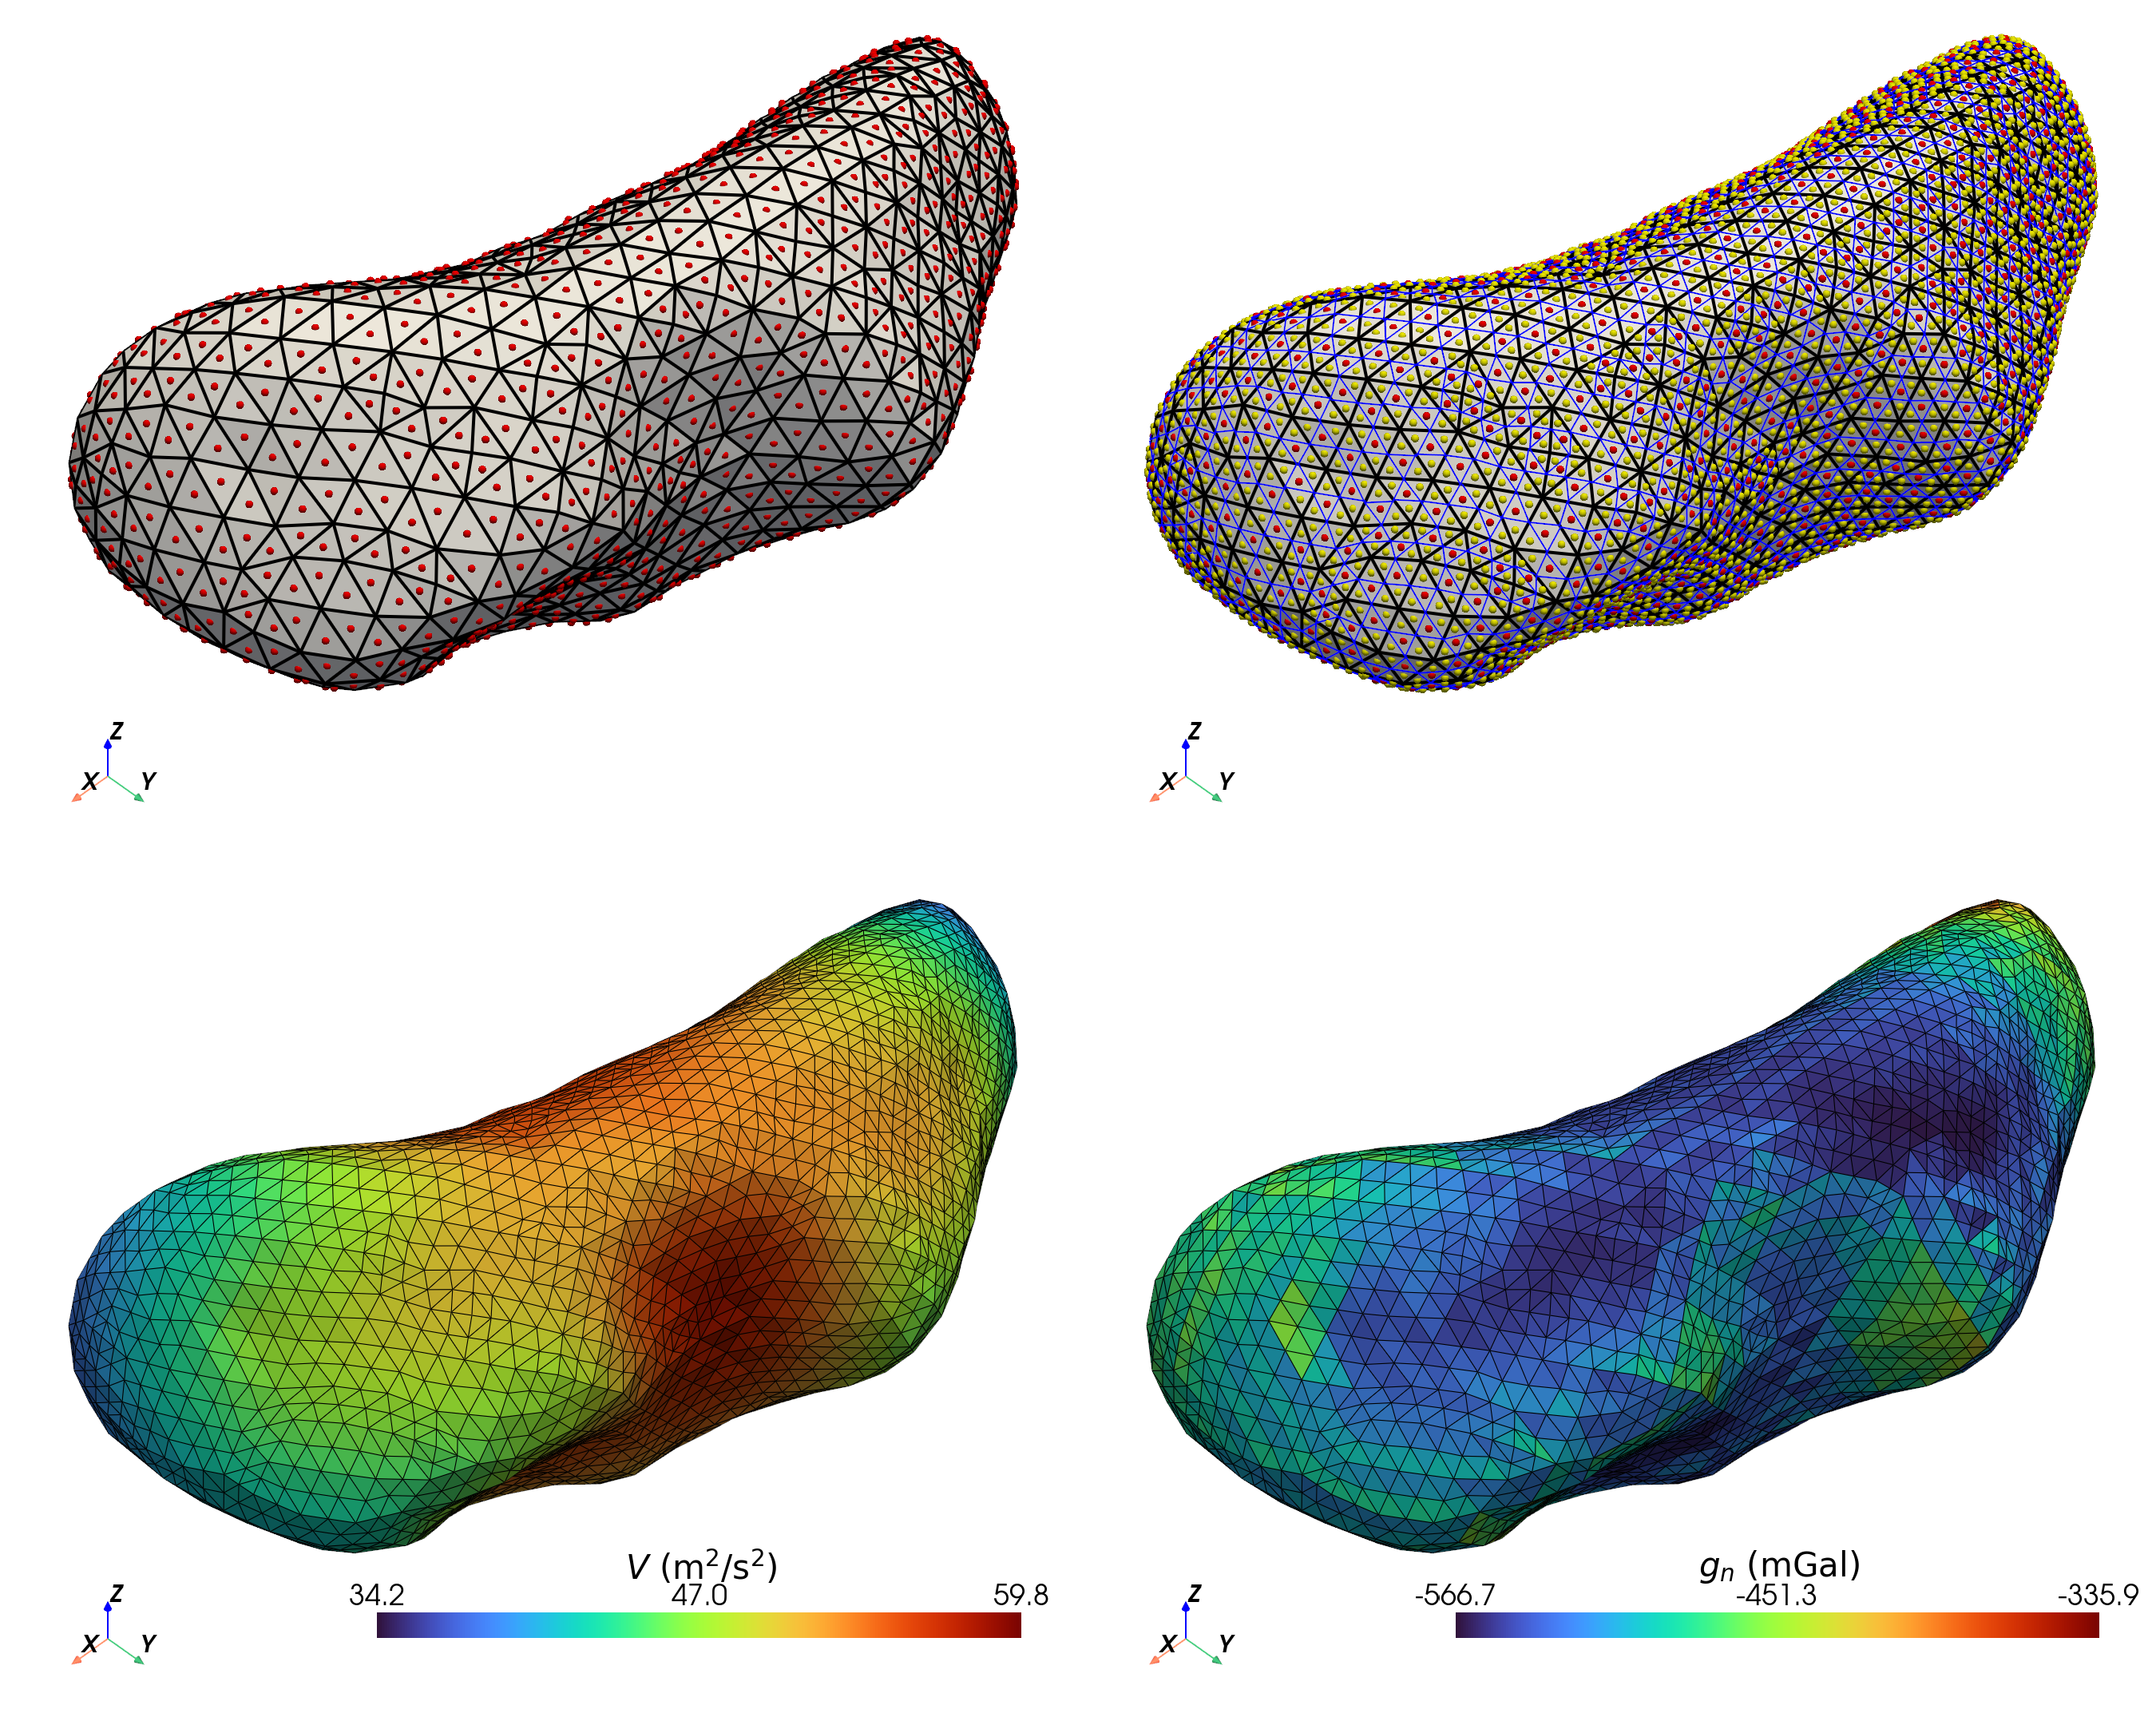
\includegraphics[width=0.95\textwidth]{Figs/EROS_Geometry.png}
    \caption{Linear refinement of the EROS shape model and surface gravity fields. Top-left: original mesh with face centers (red). Top-right: refined mesh showing new interior edges (blue) and new face centers (yellow). Bottom-left: gravitational potential $V$ on refined surface. Bottom-right: normal gravity component $g_n$.}
    \label{fig:EROS_Geometry}
\end{figure}

\clearpage
\begin{figure}
    \centering
    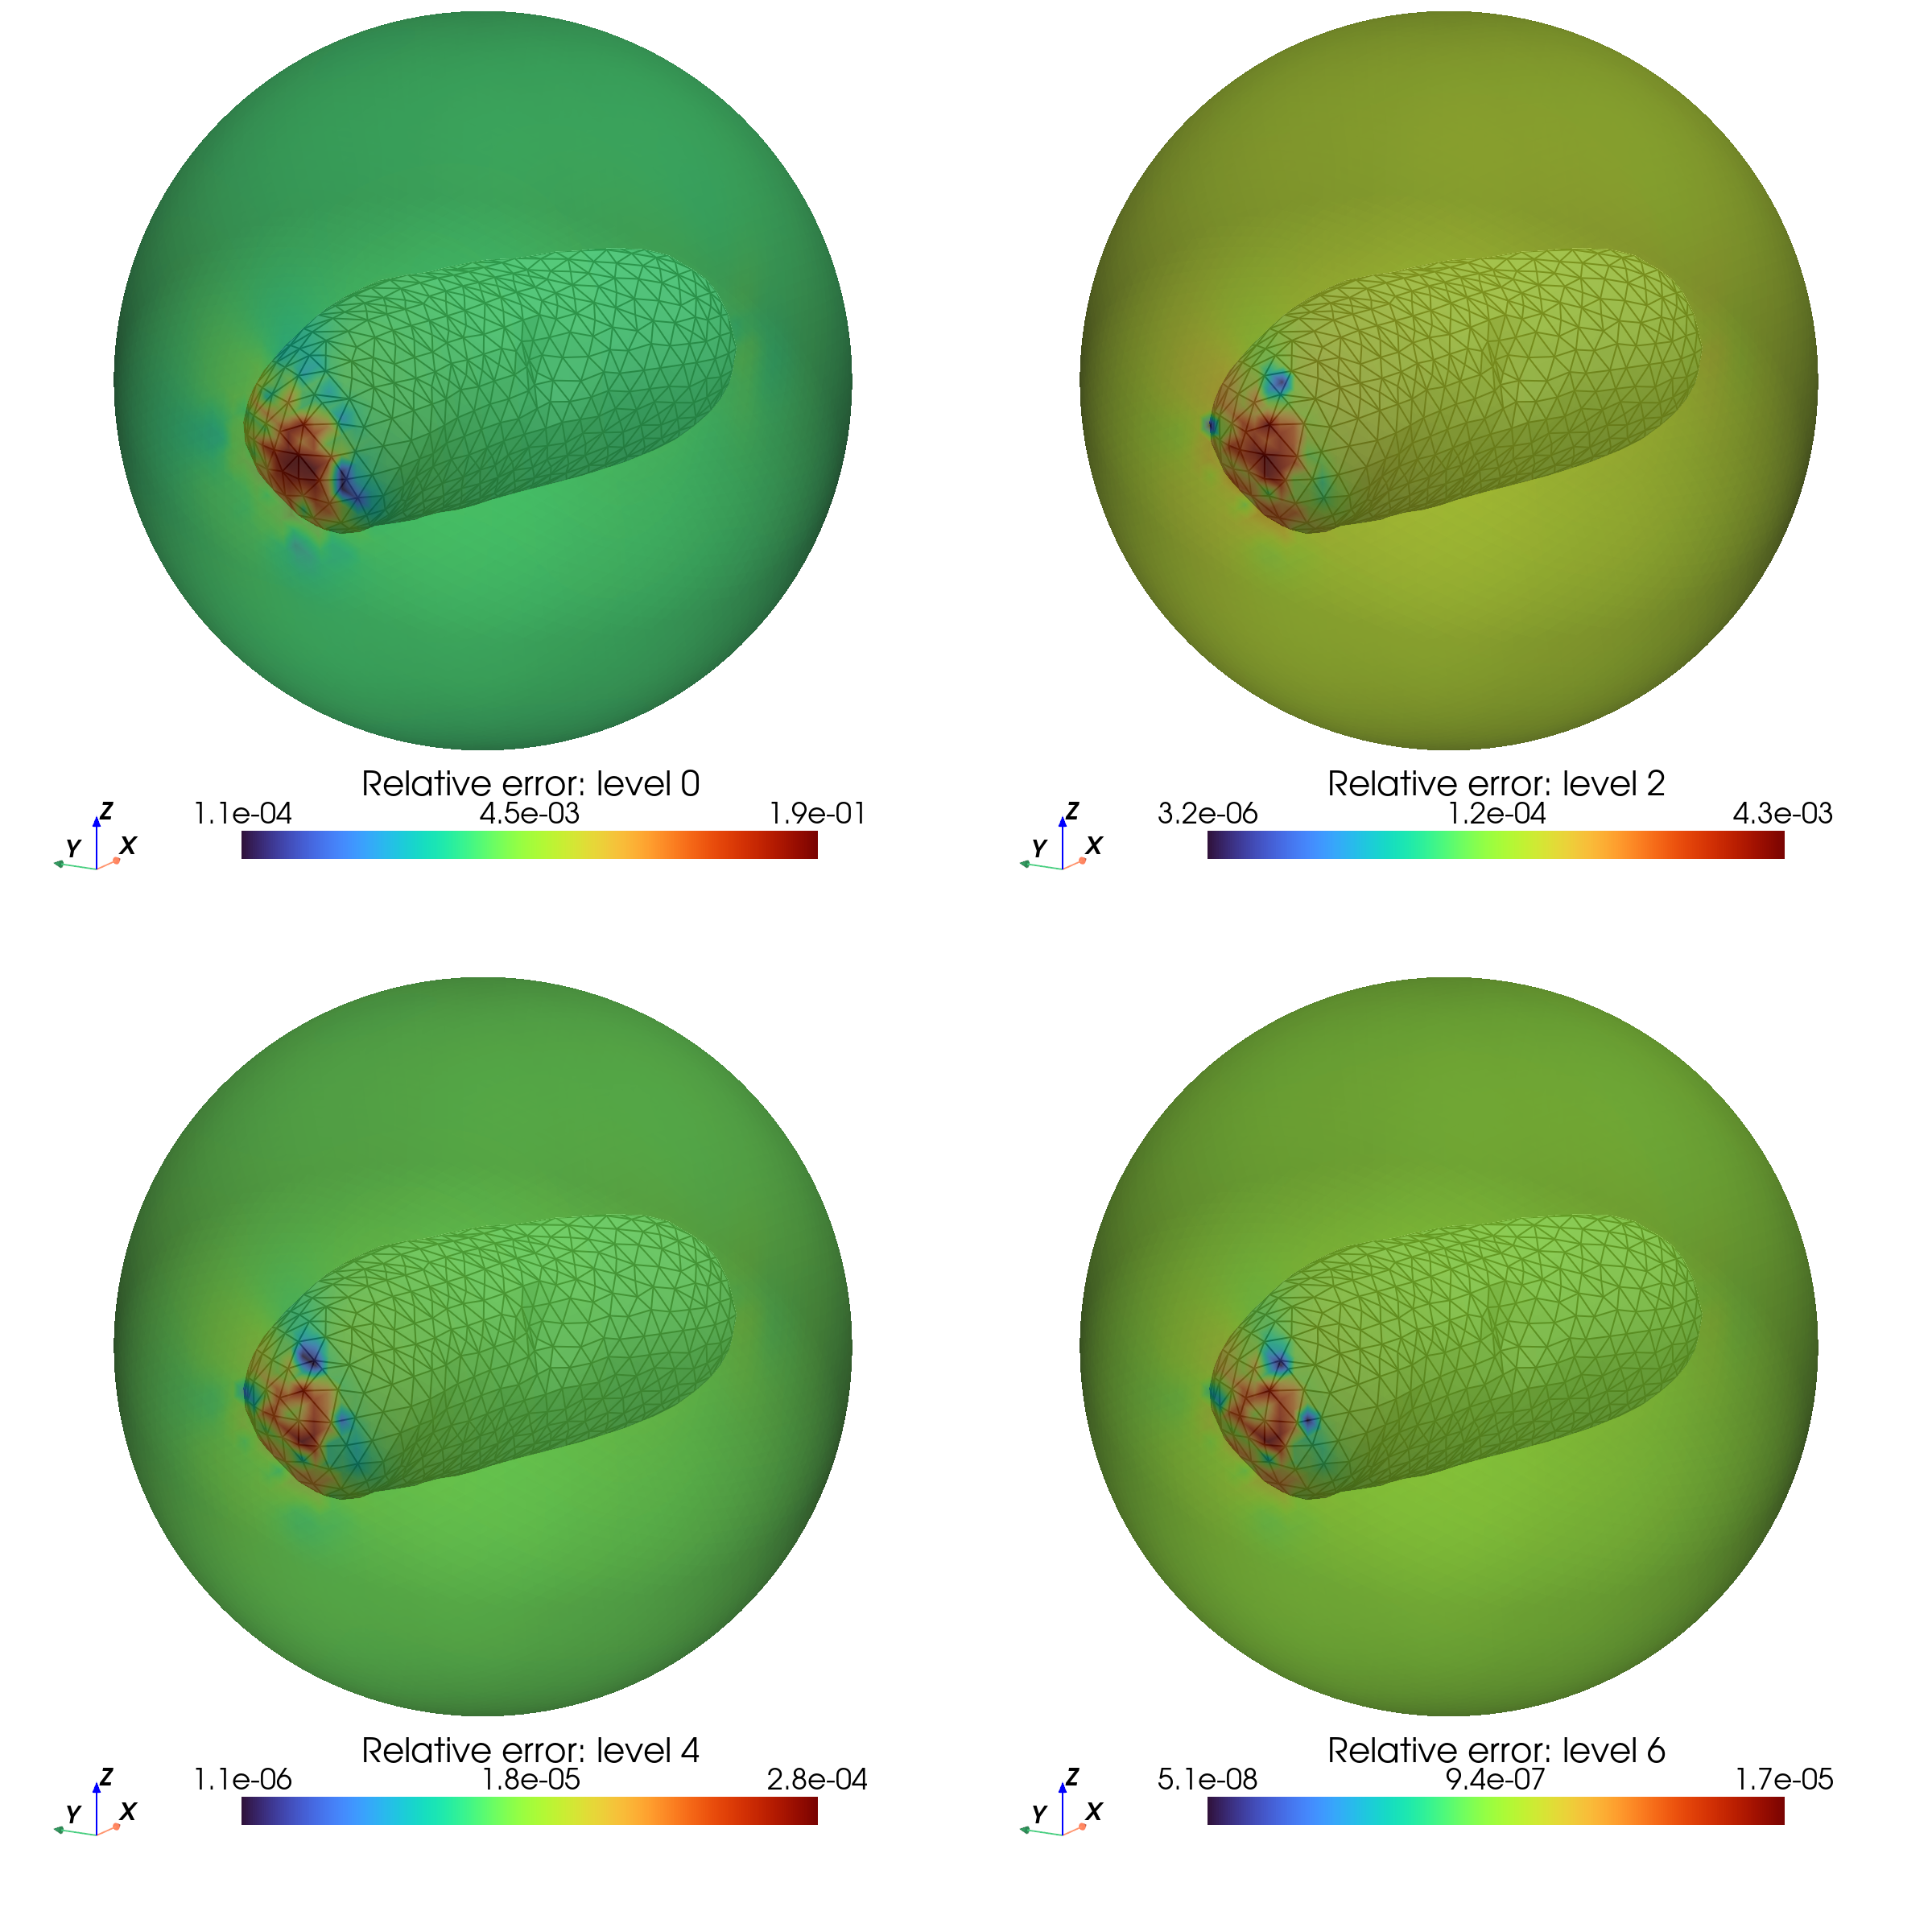
\includegraphics[width=0.95\textwidth]{Figs/EROS_ErrorMaps.png}
    \caption{Pointwise relative errors using Green's third identity approximated gravitational potential on a sphere of radius 17.8 km, shown for four mesh refinement levels. Errors are initially concentrated near the elongated tips of EROS (along $\pm x$) where the surface lies closest to the evaluation sphere, and this spatial pattern persists even at the finest resolution, albeit with dramatically reduced magnitude.}
    \label{fig:EROS_ErrorMaps}
\end{figure}

\clearpage
\begin{figure}
    \centering
    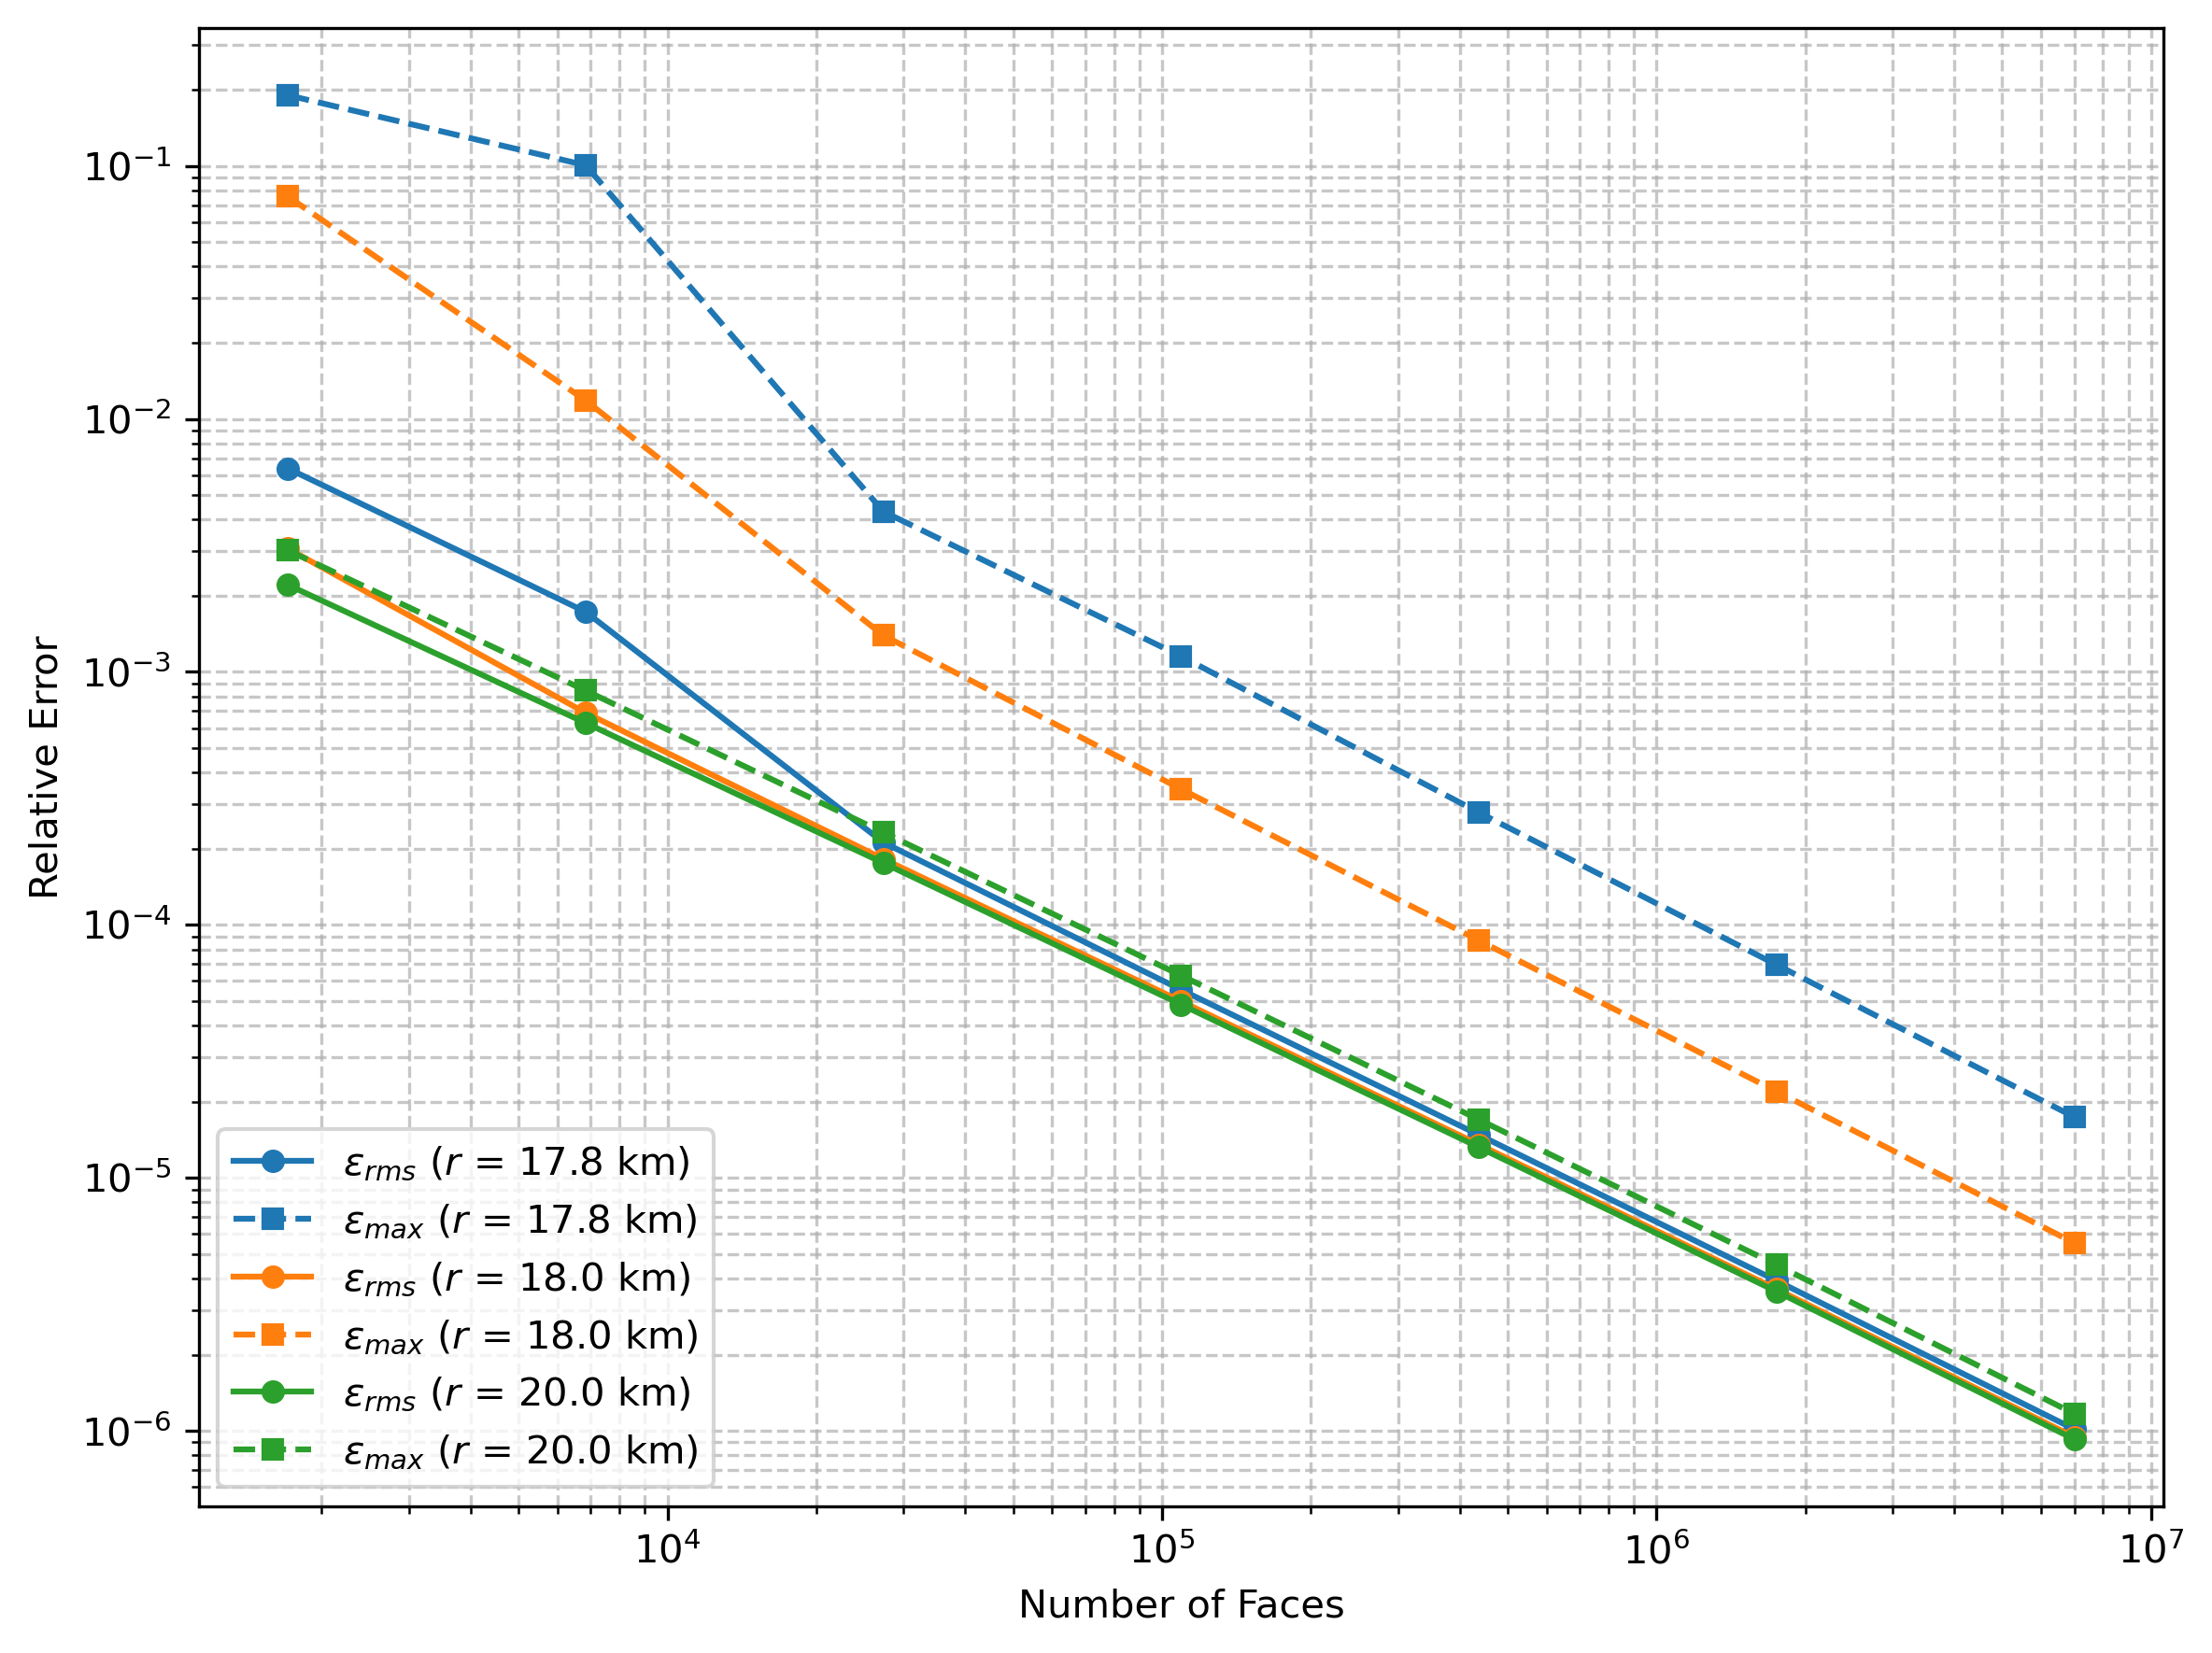
\includegraphics[width=0.95\textwidth]{Figs/EROS_Convergence.png}
    \caption{Convergence of Green's third identity approximation for EROS. Root Mean Square (RMS) relative error ($\varepsilon_{rms}$, solid lines) and maximum relative error ($\varepsilon_{max}$, dashed lines) in gravitational potential decrease with mesh refinement across three evaluation radii. Errors diminish by over three orders of magnitude as the number of faces increases from $1.7 \times 10^3$ (level 0) to $7.0 \times 10^6$ (level 6).}
    \label{fig:EROS_Convergence}
\end{figure}

\clearpage
\begin{figure}
    \centering
    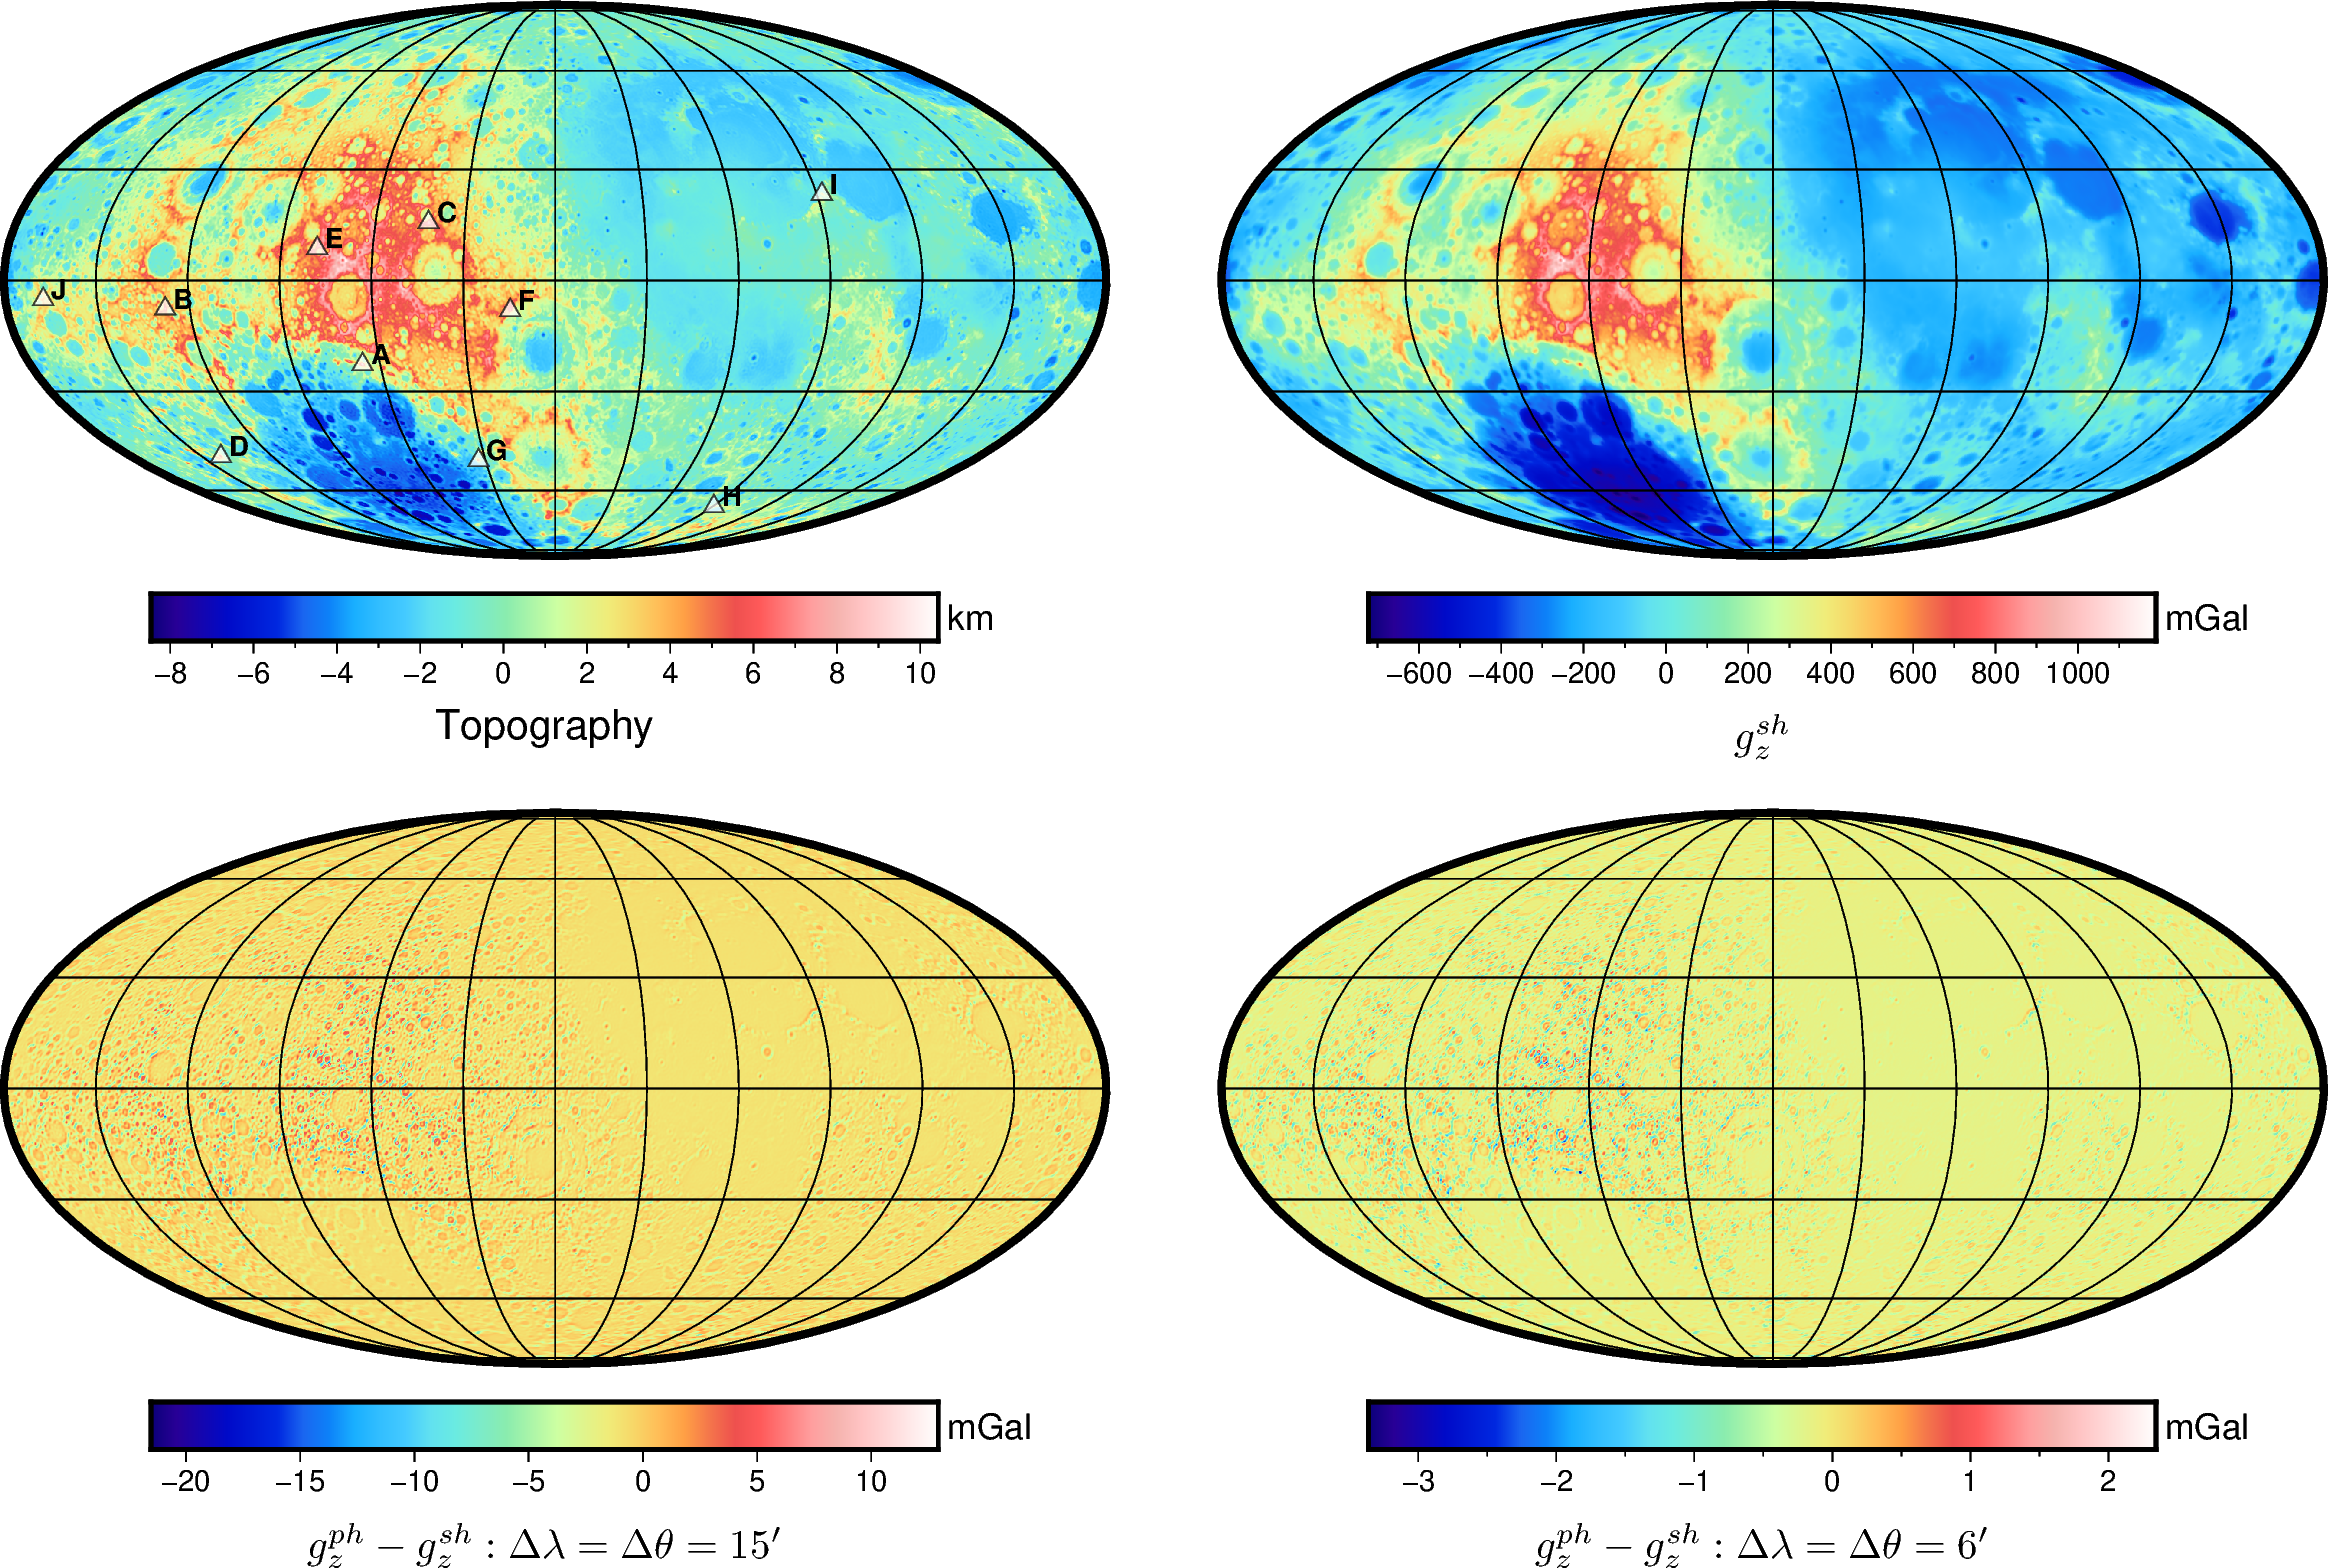
\includegraphics[width=0.95\textwidth]{Figs/Moon_TopoGz_PH_vs_SH_2.png}
    \caption{Global comparison of lunar gravity derived from spherical harmonics (SH) and polyhedral (PH) methods. Top left: Lunar topography with white triangles marking the locations of the largest $g_z$ errors in the $15$-arcmin PH-SH difference; triangle sites are separated by at least $1000$~km. Top right: Downward gravity component $g_z^{\mathrm{sh}}$ from the SH model. Bottom left: Difference $g_z^{\mathrm{ph}} - g_z^{\mathrm{sh}}$ for the $15$-arcmin PH model. Bottom right: Same difference for the $6$-arcmin PH model.}
    \label{fig:Moon_TopoGz_PH_vs_SH_2}
\end{figure}

\clearpage
\begin{figure}
    \centering
    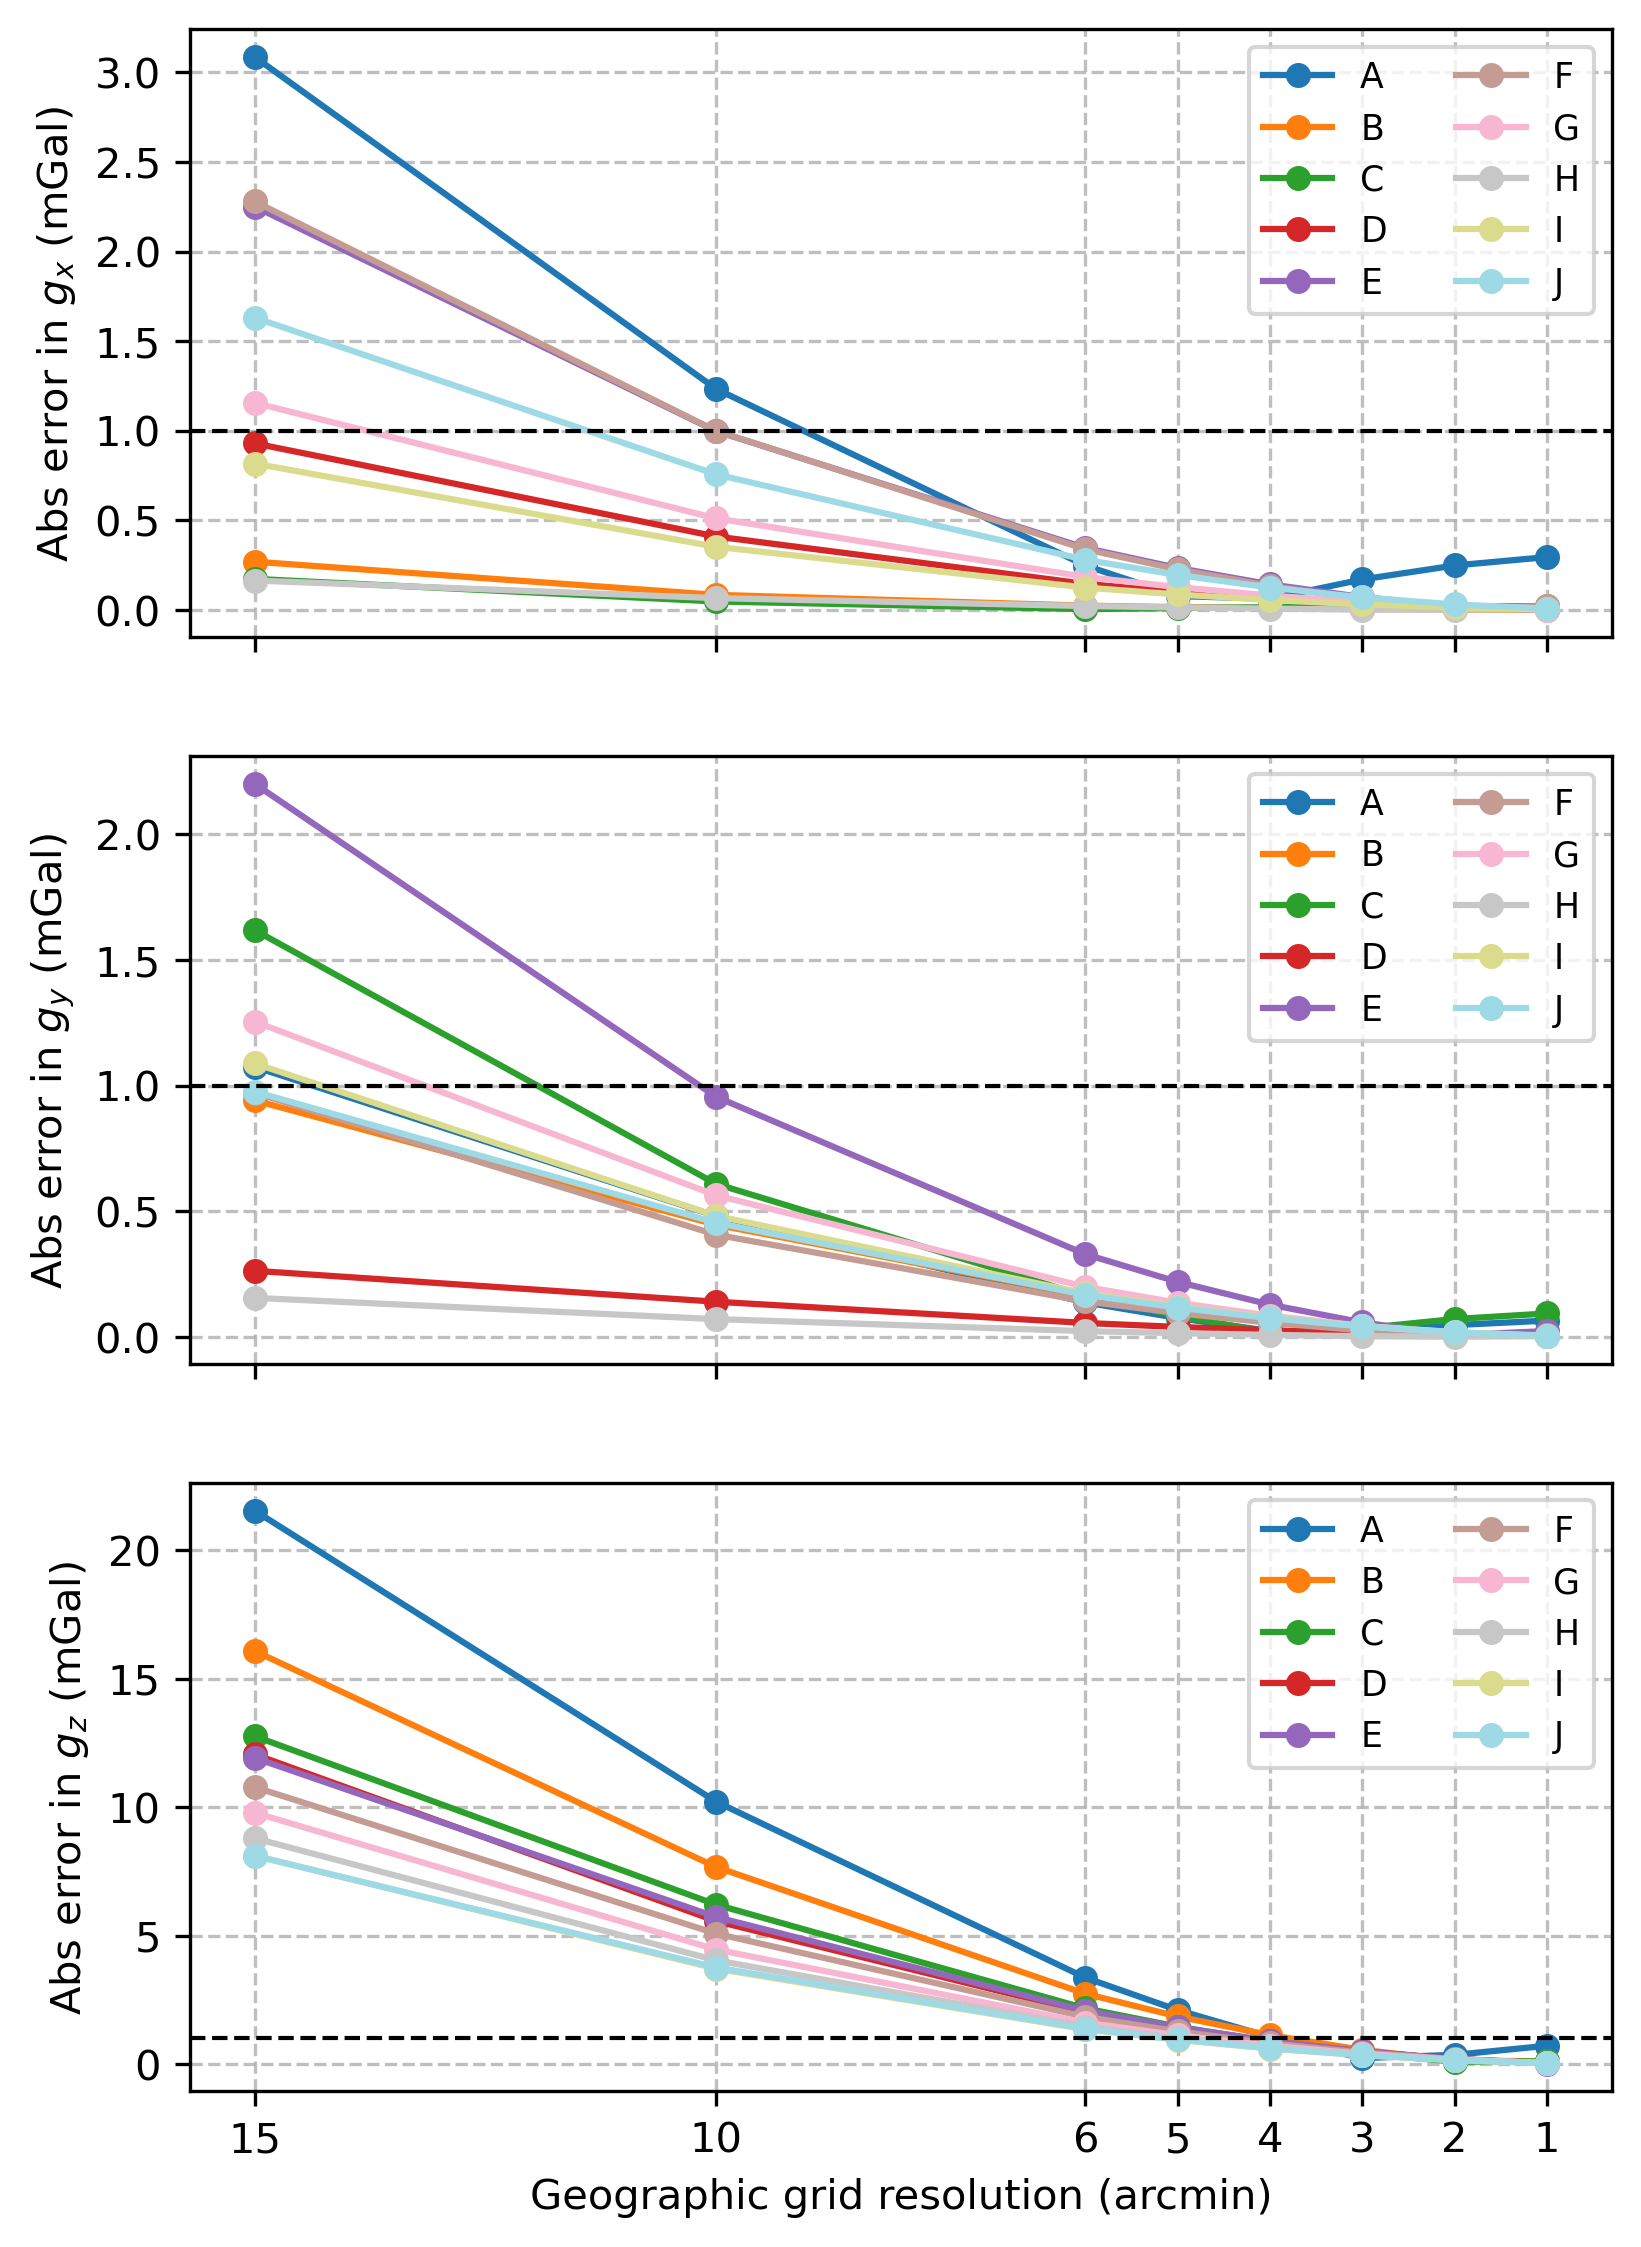
\includegraphics[width=0.75\textwidth]{Figs/Moon_TopoGxyz_PH_vs_SH_3.png}
    \caption{Absolute errors in the gravity components ($g_x$, $g_y$, $g_z$) at the ten labelled sites (A-J) identified in Figure~\ref{fig:Moon_TopoGz_PH_vs_SH_2}, plotted against polyhedral mesh resolution from $15$ to $1$ arcminute. Errors are relative to the spherical harmonic (SH) reference solution. The dashed horizontal line indicates the $1$~mGal level.}
    \label{fig:Moon_TopoGxyz_PH_vs_SH_3}
\end{figure}

\clearpage
\begin{table}[h!]
\centering
\setlength{\tabcolsep}{4.8pt}
\caption{Comparison of recursive icosahedral subdivision and triangulated regular geographic grids for approximating an ideal unit sphere. For each refinement level $n$ (with corresponding numbers of vertices $N_V$ and triangular faces $N_T$), the table reports relative surface area and volume discretization errors ($\epsilon_{\mathrm{area}}$, $\epsilon_{\mathrm{vol}}$) and the shortest and longest edge lengths ($\psi_{\mathrm{min}}$, $\psi_{\mathrm{max}}$), expressed as spherical distances in arcminutes, across levels $n = 0$ to $12$.}
\label{tab:ico_geo_sphere}
\begin{tabular}{rrrcccccccc}
\toprule
\multirow{2}{*}{$n$} &
\multirow{2}{*}{$N_{V}$} &
\multirow{2}{*}{$N_{T}$} &
\multicolumn{4}{c}{\textbf{Icosahedron}} &
\multicolumn{4}{c}{\textbf{Geographic}} \\
\cmidrule(lr){4-7} \cmidrule(lr){8-11}
& & &
$\epsilon_{\mathrm{area}}^{\mathrm{ico}}$ &
$\epsilon_{\mathrm{vol}}^{\mathrm{ico}}$ &
$\psi_{\mathrm{min}}^{\mathrm{ico}}$ &
$\psi_{\mathrm{max}}^{\mathrm{ico}}$ &
$\epsilon_{\mathrm{area}}^{\mathrm{geo}}$ &
$\epsilon_{\mathrm{vol}}^{\mathrm{geo}}$ &
$\psi_{\mathrm{min}}^{\mathrm{geo}}$ &
$\psi_{\mathrm{max}}^{\mathrm{geo}}$ \\
\midrule
0   & 12          & 20         & 2.4e-01 & 4.0e-01 & 3.8e+03 & 3.8e+03 & 2.5e-01 & 4.3e-01 & 3.6e+03 & 5.5e+03 \\
1   & 42          & 80         & 7.2e-02 & 1.3e-01 & 1.9e+03 & 2.2e+03 & 8.0e-02 & 1.5e-01 & 1.3e+03 & 3.0e+03 \\
2   & 162         & 320        & 1.9e-02 & 3.4e-02 & 8.7e+02 & 1.1e+03 & 2.3e-02 & 4.6e-02 & 3.7e+02 & 1.6e+03 \\
3   & 642         & 1280       & 4.8e-03 & 8.6e-03 & 4.1e+02 & 5.7e+02 & 6.3e-03 & 1.3e-02 & 9.9e+01 & 8.3e+02 \\
4   & 2562        & 5120       & 1.2e-03 & 2.2e-03 & 2.0e+02 & 2.8e+02 & 1.7e-03 & 3.3e-03 & 2.6e+01 & 4.2e+02 \\
5   & 10242       & 20480      & 3.0e-04 & 5.4e-04 & 9.8e+01 & 1.4e+02 & 4.2e-04 & 8.4e-04 & 6.5e+00 & 2.1e+02 \\
6   & 40962       & 81920      & 7.5e-05 & 1.4e-04 & 4.8e+01 & 7.1e+01 & 1.1e-04 & 2.1e-04 & 1.6e+00 & 1.1e+02 \\
7   & 163842      & 327680     & 1.9e-05 & 3.4e-05 & 2.4e+01 & 3.6e+01 & 2.7e-05 & 5.3e-05 & 4.1e-01 & 5.4e+01 \\
8   & 655362      & 1310720    & 4.7e-06 & 8.5e-06 & 1.2e+01 & 1.8e+01 & 6.7e-06 & 1.3e-05 & 1.0e-01 & 2.7e+01 \\
9   & 2621442     & 5242880    & 1.2e-06 & 2.1e-06 & 6.0e+00 & 8.9e+00 & 1.7e-06 & 3.4e-06 & 2.6e-02 & 1.4e+01 \\
10  & 10485762    & 20971520   & 2.9e-07 & 5.3e-07 & 3.0e+00 & 4.4e+00 & 4.2e-07 & 8.4e-07 & 6.5e-03 & 6.8e+00 \\
11  & 41943042    & 83886080   & 6.3e-08 & 1.3e-07 & 1.5e+00 & 2.2e+00 & 1.0e-07 & 2.1e-07 & 1.6e-03 & 3.4e+00 \\
12  & 167772162   & 335544320  & 2.5e-08 & 3.3e-08 & 7.5e-01 & 1.1e+00 & 2.2e-08 & 5.2e-08 & 4.0e-04 & 1.7e+00 \\
\bottomrule
\end{tabular}
\end{table}

\clearpage
\begin{table}[h!]
\centering
\caption{Statistical comparison of lunar topographic gravity vector components (in mGal) between spherical harmonic (SH) and polyhedral (PH) methods at $15^{\prime}$ and $6^{\prime}$ mesh resolutions. The components $g_x$, $g_y$, and $g_z$ represent the northward, eastward, and downward directions, respectively, in a local north-oriented coordinate system. Differences are defined as PH~$-$~SH.}
\label{tab:Moon_SH_PH_comparison}
\begin{tabular}{lcccccc}
\toprule
Method & Component & min & max & mean & std \\
\midrule
\multirow{3}{*}{SH} 
   & $g_x$ & $-488.8082$ & $933.4147$ & $10.3820$ & $154.3514$ \\
   & $g_y$ & $-551.9941$ & $606.5575$ & $0.0197$  & $150.2317$ \\
   & $g_z$ & $-721.8590$ & $1189.4579$ & $-35.0952$ & $246.4136$ \\
\midrule
\multirow{3}{*}{PH ($15^{\prime}$)} 
   & $g_x$ & $-486.9639$ & $926.2217$ & $10.3856$ & $154.2915$ \\
   & $g_y$ & $-548.6204$ & $605.3110$ & $0.0197$  & $150.2471$ \\
   & $g_z$ & $-721.7818$ & $1182.6341$ & $-36.0165$ & $246.2114$ \\
\midrule
\multirow{3}{*}{Diff ($15^{\prime}$)} 
   & $g_x$ & $-12.0679$ & $12.5141$ & $0.0033$ & $0.8889$ \\
   & $g_y$ & $-11.6858$ & $10.1128$ & $-0.0000$ & $0.7200$ \\
   & $g_z$ & $-21.5349$ & $12.9305$ & $-0.9188$ & $1.1335$ \\
\midrule
\multirow{3}{*}{PH ($6^{\prime}$)} 
   & $g_x$ & $-488.5107$ & $932.2260$ & $10.3829$ & $154.4438$ \\
   & $g_y$ & $-551.4422$ & $606.3592$ & $0.0197$  & $150.3391$ \\
   & $g_z$ & $-721.8638$ & $1187.8352$ & $-35.2429$ & $246.3798$ \\
\midrule
\multirow{3}{*}{Diff ($6^{\prime}$)} 
   & $g_x$ & $-1.9898$ & $2.0846$ & $0.0006$ & $0.1456$ \\
   & $g_y$ & $-2.1117$ & $1.6070$ & $-0.0000$ & $0.1181$ \\
   & $g_z$ & $-3.3589$ & $2.3430$ & $-0.1474$ & $0.1888$ \\
\bottomrule
\end{tabular}
\end{table}

\clearpage
\bibliographystyle{seg}
\bibliography{Paper_WerSch_Geophy}


\end{document}
